\section{Beyond short-run prices: spatial markets, repositioning and investment}\label{sec:11-beyond}

The merger simulations of \cref{sec:11-simulation} hold three things fixed. They fix the set of products and
their characteristics. They fix each firm's capacity. They also summarize substitution with a demand system in
which location plays no explicit role. This section studies three papers that relax one of these restrictions
each. \citet{Houde2012} builds the geography of a retail market into demand and checks a merger simulation against
a difference-in-differences estimate of the same merger. \citet{Sweeting2010} documents how merging radio stations
change their programming, a dimension that a price-only analysis ignores. \citet{Pesendorfer2003} models capacity
investment and uses investment choices to infer the cost savings that mergers produced.

\subsection{Spatial competition and the Ultramar-Sunoco transaction: Houde (2012)}\label{sec:11-houde}

\casehead{Question}
How much does a merger of retail outlets raise prices when consumers are mobile? \citet{Houde2012} argues that the
relevant location of a gasoline buyer is the whole route she drives between home and work, not her home address.
Two stations far apart can then be close substitutes if many commuters pass both. Substitution depends on the road
network and on the direction of traffic. The paper asks two questions. Does a demand model built on commuting paths
fit the data better than the usual home-address model? Does a merger simulation based on it predict the price
effects of an observed merger, as measured by a retrospective difference-in-differences study?

The second question matters for the methodological debate of \cref{sec:11-retro,sec:11-bv}. A retrospective
estimate is transparent but tied to one sample and one control group. A simulation can evaluate any counterfactual
but rests on a demand model. Comparing the two on the same merger is a validation exercise in the spirit of
\citet{LaLonde1986}, who compared nonexperimental estimators with an experimental benchmark. Here the demand model is
estimated without the supply restrictions that the merger imposes, so the comparison is a true out-of-sample test.

\casehead{Setting}
The market is the Quebec City census metropolitan area between 1991 and 2001. Five major brands were present:
Shell, Esso, Petro-Canada, Irving and Ultramar. Ultramar was the leading chain and the only firm with a refinery
near the city. The 1990s brought a large reorganization of North American gasoline retailing. Technology raised the
efficient size of stations, the value of small repair garages fell, and new environmental rules forced owners to
replace underground storage tanks. The number of stations in Quebec City fell by 30 percent, from 382 in 1991 to
283 in December 2001, mostly through exit by stations of the major chains \citep[p.~2152]{Houde2012}.

Two further facts shape the analysis. Prices are tightly clustered. Over most of the period the interquartile range
of prices was below one cent per litre (cpl), about 1.5 percent of the average price. Retail margins over the rack
price, the wholesale price posted at the terminal, ranged between 8 and 15 percent of the price for most of the
period. There were also two price wars. The first, in the summer of 1996, followed excess capacity and a low-price
guarantee campaign by Ultramar. In 2000 average margins fell to zero after several stations priced at a regulated
price floor, introduced by a provincial law of December 1996 \citep[pp.~2152--2153]{Houde2012}.

\casehead{Data}
The station data come from Kent Marketing, a survey firm that visits every station at the end of each survey period
and reads the volume sold off the pump meters. The panel has 46 bimonthly periods between 1991 and 2001, with only the
fourth period observed in the first four years. It contains 14,263 station-period observations on 429 station sites.
Observed characteristics include the size of the convenience store, a repair-shop indicator, the numbers of
service islands and pumps, opening hours, brand, type of service and a car wash. The price is the posted unleaded
price on the survey day, deflated by the regional consumer price index. Average volume was 4,934 litres per day
(standard deviation 3,289), and the average real price was 63.83 cpl (Table~1). About 8 percent of the sample
stations refused the survey in some or all periods. Their characteristics and prices are observed, and Houde imputes
their volumes by linear regression on neighborhood shares, predicted traffic, population density, location, prices,
characteristics and lagged sales \citep[p.~2151, n.~12]{Houde2012}.

Table~1 also shows how much the stations changed over the decade. From fall 1991 to fall 2001 average volume rose from
3,949 to 6,271 litres per day, and the number of pumps from 7.77 to 11.37. The share of full-service stations fell
from 0.54 to 0.28. The average absolute deviation of a station's price from the period mean fell from 0.90 to 0.13 cpl,
as most stations came to post the modal price \citep[p.~2152]{Houde2012}.

The geography comes from three sources. A road network with more than 30,000 street segments gives travel times,
and a shortest-path algorithm gives each commuter's route. Origin-destination surveys from 1991, 1996 and 2001 give
the number of commuters between traffic zones, by purpose and mode. Census and labor-force data give the population
and the income distribution of each residential area. Commuters who cross the city on highways are proxied by
occupied hotel rooms. Before estimating any model, \citet[Figure 2]{Houde2012} compares station sales with two
crude predictions. If consumers buy at random from stations within half a minute of their commuting path, predicted
and observed shares have a correlation near 0.3 in every period. If they buy at random near home, the correlation is
near zero or negative.

\casehead{Model}
Consumer $i$ commutes from home location $s_i$ to work location $d_i$ along the fastest route $r(s_i, d_i)$. The
route takes time $t(s_i,d_i)$ and covers $m(s_i,d_i)$ kilometers. Station $j$ sits at location $l_j$. The consumer
buys from one of the $J$ stations or takes the outside option $j = 0$, which is to commute without a car. Her
indirect utility is \citep[eq.~(1)]{Houde2012}
\begin{equation}\label{eq:11-houde-u}
u_{ij} =
\begin{cases}
x_j\beta + (\bar\alpha + \alpha_y y_i)\,p_j + \lambda_1\,\mathcal{D}\big(r(s_i,d_i), l_j\big) + \xi_j + \epsilon_{ij},
& j = 1,\dots,J,\\[2pt]
-\lambda_0\,\mathit{Long}(s_i,d_i) + \epsilon_{i0}, & j = 0.
\end{cases}
\end{equation}
Here $x_j$ collects station characteristics, brand and period dummies, $\xi_j$ is unobserved station quality,
$y_i$ is the log hourly wage, and $\epsilon_{ij}$ is type-I extreme value. The indicator $\mathit{Long}(s,d)$
equals one when home and work lie in different traffic zones. Houde writes $C(s,d)$ for it, and we rename it to avoid
confusion with cost functions. Long commuters are more likely to drive, so we expect
$\lambda_0 > 0$. The paper writes the price term as $+(\bar\alpha + \alpha_y y_i)\,p_j$ (eq.~(1) and p.~2157), and
the estimated $\bar\alpha$ is negative (Table~3). In the sign convention of this book the consumer's price
coefficient is therefore $\alpha_i = -(\bar\alpha + \alpha_y y_i)$. The symbols $\lambda_0$ and $\lambda_1$ are local
to this subsection.

The novel object is the \emph{detour} $\mathcal{D}$. It measures the extra driving time needed to stop at $l$ on the
way from $s$ to $d$:
\begin{equation}\label{eq:11-houde-detour}
\mathcal{D}\big(r(s,d), l\big) = t(s,l) + t(l,d) - t(s,d).
\end{equation}
A station on the route costs no extra time. The standard single-address model is nested as the special case in which
the consumer starts and ends at home, $\mathcal{D}^h(s,l) = 2\,t(s,l)$. Transport costs make utility fall with the
detour, so we expect $\lambda_1 < 0$. \Cref{fig:11-detour} illustrates the difference between the two metrics.

\begin{figure}[htbp]
\centering
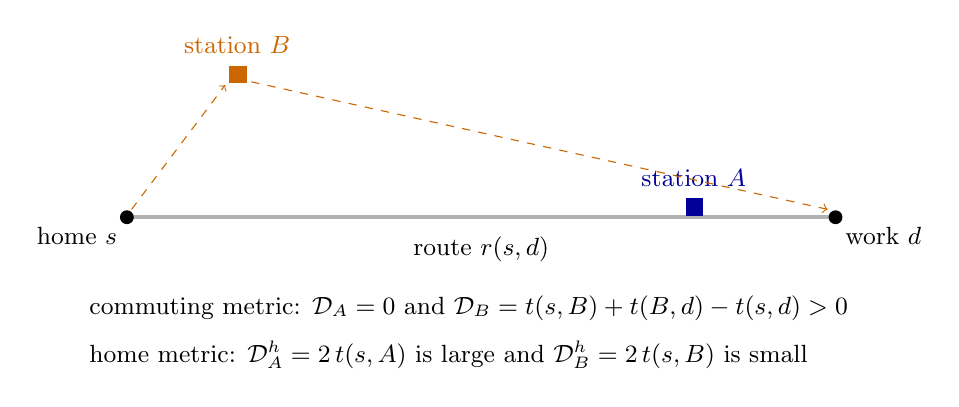
\begin{tikzpicture}[every node/.style={font=\small}]
  \draw[line width=1.6pt, gray!60] (0,0) -- (9,0);
  \node[below] at (4.5,-0.12) {route $r(s,d)$};
  \fill (0,0) circle (2.5pt) node[below left] {home $s$};
  \fill (9,0) circle (2.5pt) node[below right] {work $d$};
  \fill[blue!60!black] (7.1,0.02) rectangle +(0.22,0.22);
  \node[above, blue!60!black] at (7.2,0.27) {station $A$};
  \fill[orange!80!black] (1.3,1.7) rectangle +(0.22,0.22);
  \node[above, orange!80!black] at (1.4,1.95) {station $B$};
  \draw[dashed, orange!80!black, ->] (0.06,0.1) -- (1.25,1.68);
  \draw[dashed, orange!80!black, ->] (1.58,1.72) -- (8.9,0.1);
  \node[anchor=west] at (-0.6,-1.15) {commuting metric: $\mathcal{D}_A = 0$ and $\mathcal{D}_B = t(s,B) + t(B,d) - t(s,d) > 0$};
  \node[anchor=west] at (-0.6,-1.75) {home metric: $\mathcal{D}^h_A = 2\,t(s,A)$ is large and $\mathcal{D}^h_B = 2\,t(s,B)$ is small};
\end{tikzpicture}
\caption{Two distance metrics in the demand model of \citet{Houde2012}. Station $A$ lies on the commuter's route
near her workplace, so it requires no detour although it is far from home. Station $B$ is close to home but off the
route. The commuting metric ranks $A$ closer, and the home metric ranks $B$ closer.}
\label{fig:11-detour}
\end{figure}

Gasoline demand is inelastic at the individual level. A consumer of type $(s,d)$ who buys at all buys
$\bar q(s,d) = \bar q_0 + \bar q_1 m(s,d)$ litres, where $\bar q_1$ is fixed at the average fuel use of a city car and
$\bar q_0$ is estimated. Houde writes $c_0$ and $c_1$ for these parameters. The text fixes $\bar q_1$ at 0.10 litres
per kilometer (p.~2156), while Tables~3 and 4 list the fixed value as 0.2. The paper does not reconcile the two
numbers. With $T_{s,d}$ commuters between $s$ and
$d$, market size is $M = \sum_s\sum_d \bar q(s,d)\,T_{s,d}$ (eq.~(2)). Write the inside utility net of the
logit shock as $V_{ij} = \delta_j + (\bar\alpha + \alpha_y y_i)p_j + \lambda_0\mathit{Long}(s_i,d_i) +
\lambda_1\mathcal{D}(r(s_i,d_i),l_j)$, where $\delta_j = x_j\beta + \xi_j$. Adding $\lambda_0\mathit{Long}$ to every
inside option normalizes the outside utility to zero. The choice probability and station demand are (eqs.~(3)--(4))
\begin{equation}\label{eq:11-houde-demand}
P_{ij} = \frac{\exp(V_{ij})}{1 + \sum_{k=1}^{J}\exp(V_{ik})},
\qquad
Q_j(p) = \sum_s\sum_d \bar q(s,d)\, T_{s,d}\int P_{j}\big(r(s,d), y\big)\, dF(y \mid s),
\end{equation}
where $F(y \mid s)$ is the wage distribution in home area $s$. The integral is computed by simulation.

Houde also estimates a discrete-continuous alternative, in which each consumer's quantity responds to price through
Roy's identity. The demand results are unchanged. The supply results, however, imply that firms behave as strategic
substitutes after a simulated merger, so that competitors cut their prices. Houde attributes this to conditional
demand that is inelastic for most consumers and treats the functional form as inaccurate \citep[p.~2157,
n.~24]{Houde2012}.

The commuting structure determines substitution through the following algebra. Write $a_i = \bar\alpha + \alpha_y
y_i < 0$ and let $\sum_i h_i(\cdot)$ denote the sum over consumer types, with weights $h_i = \bar q(s_i,d_i)
T_{s_i,d_i}\,\dd F(y_i \mid s_i)$. The logit derivatives are $\frac{\partial P_{ij}}{\partial p_j} = a_i P_{ij}(1 -
P_{ij})$ and $\frac{\partial P_{ik}}{\partial p_j} = -a_i P_{ij}P_{ik}$. Summing over types gives the diversion
ratio from $j$ to $k$ of \cref{def:04-diversion}:
\begin{align}
D_{jk}
= -\dfrac{\frac{\partial Q_k}{\partial p_j}}{\frac{\partial Q_j}{\partial p_j}}
&=\frac{\sum_i h_i (-a_i) P_{ij} P_{ik}}{\sum_i h_i (-a_i) P_{ij}(1 - P_{ij})} \notag\\
&= \sum_i \underbrace{\frac{h_i (-a_i) P_{ij}(1 - P_{ij})}{\sum_{i'} h_{i'} (-a_{i'}) P_{i'j}(1 -
P_{i'j})}}_{\text{weight of type } i}\; \frac{P_{ik}}{1 - P_{ij}} . \label{eq:11-houde-diversion}
\end{align}
For each type the diversion is the logit ratio $\frac{P_{ik}}{1 - P_{ij}}$ of \cref{ch:logit}, proportional to $k$'s
share. Aggregate diversion averages these ratios with weights that are large for the types who buy at $j$ and are
price sensitive. Station $k$ therefore captures much of $j$'s lost volume when the commuters who patronize $j$ also
pass close to $k$. This is how the road network enters the substitution matrix, and why stations far apart can be
close substitutes. A home-address model weights types by where they live and misses this channel.

\casehead{Estimation}
The parameters $(\bar q_0, \lambda_0, \lambda_1, \alpha_y, \bar\alpha, \beta)$ are estimated by the nested fixed point
GMM method of \citet{Berry1994} and \citet{BerryLevinsohnPakes1995} (\cref{ch:blp}). Two sets of moments are combined.
The first follows \citet{Nevo2001} and uses station-location fixed effects. Write $\xi_{jt} = \bar\xi_j +
\tilde\xi_{jt}$, where $\bar\xi_j$ is the permanent quality of the site (ease of access, side of the street) and
$\tilde\xi_{jt}$ a transitory shock. With $\tilde w_{jt}$ the within-station deviation of a variable, the moments are
(eq.~(5))
\begin{equation}\label{eq:11-houde-m1}
\bar g^1_n(\theta) = \frac{1}{n}\sum_{j,t}\tilde\xi_{jt}(\theta)\,\tilde W^1_{jt},
\end{equation}
where $\tilde W^1_{jt}$ contains the within-transformed station characteristics, the excluded instruments $z_{jt}$
and period dummies.

The second set is a micro moment that disciplines the outside option. The 2001 origin-destination survey reports
the share of commuters between each pair of zones who drive. The model predicts the same share as one minus the
probability of the outside option, $U_{sd}(\theta)$. With $\hat U_{sd}$ the observed share, the moments are
(eq.~(6))
\begin{equation}\label{eq:11-houde-m2}
\bar g^2_{n_2}(\theta) = \frac{1}{n_2}\sum_{s,d}\big(U_{sd}(\theta) - \hat U_{sd}\big)W^2_{sd},
\end{equation}
with $W^2_{sd}$ a constant, the long-commute indicator and simulated income. These moments force the model to
reproduce a reduced-form regression estimated on 3,000 simulated survey respondents (eq.~(7)):
\begin{equation}\label{eq:11-houde-carreg}
\hat U_i = \underset{(0.033)}{0.247} + \underset{(0.0141)}{0.0495}\; y_i + \underset{(0.0163)}{0.315}\;
\mathit{Long}_i, \qquad R^2 = 0.47 .
\end{equation}
The intercept pins down $\bar q_0$ and hence market size, the income slope pins down $\alpha_y$, and the
long-commute slope pins down $\lambda_0$. The weighting matrix allows for serial and spatial correlation in
$\tilde\xi_{jt}$. With 46 periods and more than 300 stations, the inner loop is costly. Houde inverts demand with a
derivative-free quasi-Newton algorithm, which is faster than the contraction mapping of
\citet{BerryLevinsohnPakes1995}. The inner-loop tolerance is $10^{-12}$, tightened to $10^{-14}$ for the standard
errors \citep[p.~2160, n.~27]{Houde2012}.

\casehead{Instruments and identification}
Two parameters need excluded variation: the price coefficient $\bar\alpha$ and the transport cost $\lambda_1$. Prices
are endogenous because firms see $\xi_{jt}$ and because frequent price changes make the survey-day price a noisy
measure of the price that generated the period's volume. The transport cost enters nonlinearly, and it is identified
by how a station's sales respond to changes in its neighbors.

The identifying assumption is that the transitory quality shock $\tilde\xi_{jt}$ evolves independently of the
characteristics of nearby stations, conditional on location fixed effects. The industry reorganization supplies the
variation. Stations closed, opened and were rebuilt for reasons of technology and regulation that were unrelated to
local demand shocks. Entry, exit and remodeling involve large sunk costs, so they plausibly respond to $\bar\xi_j$
but not to $\tilde\xi_{jt}$. Cross-sectional versions of this argument, which assume that location quality is
independent of neighbors' characteristics, would bias the transport cost toward zero if stations locate at
high-traffic, high-quality sites \citep[p.~2160]{Houde2012}.

Competitors' characteristics are weak instruments for price, because cross-sectional price dispersion is small. Rack
prices vary mostly over time and are absorbed by period effects. Houde therefore exploits small differences in the
posted rack prices of two suppliers. Sunoco supplied the Quebec City terminal until 1997, and the independent
wholesaler Olco took over afterward. The instruments interact the Sunoco and Olco rack prices with indicators for a
Sunoco or Olco station in the neighborhood of station $j$. Table~2 of the paper defines four instrument sets.
Specification (1) uses the count and average size of competitors on the same street and the average competitor size
within 0.1, 0.33 and 1 kilometer (5 instruments). Specification (2) uses the rack-price interactions (4
instruments). Specification (3) combines the two, and specification (4) adds the fractions of competitors with
various amenities (25 instruments in that set). Two stations share a street if they have a street in common and
are within five minutes of each other. The first-stage F-statistics exceed 10 for specifications (2) and (3).

\casehead{Demand results}
\Cref{tab:11-houde-demand} reproduces the estimates of the multi-address (commuting) model and of the single-address
(home) model. The two models differ most in the transport cost. In the commuting model $\lambda_1$ is negative, large
and precise, except in specification (2), which uses only the cost instruments. In the home model it is positive in
every specification, so consumers would prefer stations farther from home. The correlations in Figure~2 of the paper
explain the sign. Large stations sit at the intersections of major commuting routes, often far from where people live,
so the home model can rationalize their sales only with a small or positive transport cost.

\begin{table}[htbp]
\centering
\caption{Demand estimates for Quebec City gasoline stations}
\label{tab:11-houde-demand}
\begin{threeparttable}
\small
\begin{tabular}{@{}lcccc@{}}
\toprule
 & (1) & (2) & (3) & (4) \\
\midrule
\multicolumn{5}{@{}l}{\emph{Panel A. Multi-address (commuting) model, Table 3}} \\
Minimum consumption $\bar q_0$ & 4.5746 & 4.5290 & 4.5582 & 4.5035 \\
 & (0.0334) & (0.0442) & (0.0299) & (0.0242) \\
Income $\alpha_y$ & 0.0396 & 0.1082 & 0.0474 & 0.1677 \\
 & (0.0307) & (0.0809) & (0.0327) & (0.0482) \\
Long commuters $\lambda_0$ & 1.4972 & 1.4356 & 1.4768 & 1.3891 \\
 & (0.0326) & (0.0683) & (0.0299) & (0.0432) \\
Transportation cost $\lambda_1$ & $-1.2777$ & $-0.5642$ & $-1.0004$ & $-0.3961$ \\
 & (0.537) & (0.29) & (0.291) & (0.0909) \\
Price $\bar\alpha$ & $-0.2181$ & $-0.1687$ & $-0.1974$ & $-0.1490$ \\
 & (0.0767) & (0.033) & (0.0378) & (0.0233) \\
Median travel cost (cpl per minute) & 5.886 & 3.398 & 5.098 & 2.733 \\
$J$-statistic (degrees of freedom) & 3.07 (3) & 1.22 (2) & 6.06 (7) & 40.5 (27) \\
\addlinespace
\multicolumn{5}{@{}l}{\emph{Panel B. Single-address (home) model, Table 4}} \\
Minimum consumption $\bar q_0$ & 5.0992 & 5.0399 & 5.1246 & 4.9940 \\
 & (0.158) & (0.0965) & (0.0691) & (0.0706) \\
Income $\alpha_y$ & $-0.8433$ & $-0.6463$ & $-0.9318$ & $-0.4574$ \\
 & (0.87) & (0.409) & (0.36) & (0.226) \\
Long commuters $\lambda_0$ & 3.6236 & 2.9233 & 3.9919 & 2.4657 \\
 & (2.53) & (1.07) & (1.06) & (0.534) \\
Transportation cost $\lambda_1$ & 0.5556 & 0.4235 & 0.6152 & 0.3181 \\
 & (0.519) & (0.235) & (0.211) & (0.126) \\
Price $\bar\alpha$ & $-0.1498$ & $-0.0918$ & $-0.1054$ & $-0.0630$ \\
 & (0.0543) & (0.0252) & (0.0275) & (0.0176) \\
Median travel cost (cpl per minute) & $-3.258$ & $-3.933$ & $-4.793$ & $-4.284$ \\
$J$-statistic (degrees of freedom) & 10.2 (3) & 3.83 (2) & 14.2 (7) & 60.6 (27) \\
\addlinespace
5 percent $\chi^2$ threshold & 7.82 & 5.99 & 14.1 & 40.1 \\
\bottomrule
\end{tabular}
\begin{tablenotes}[flushleft]
\footnotesize
\item Notes: Reproduced from \citet[Tables 3 and 4]{Houde2012}, with the paper's signs (a negative $\bar\alpha$ means
that utility falls with price, a negative $\lambda_1$ that it falls with the detour). Standard errors robust to serial
and spatial correlation in parentheses. The commuting-distance coefficient $\bar q_1$ is fixed. Both tables list it as
0.2, although the text fixes it at 0.10 litres per kilometer (p.~2156). The income row is the coefficient on the log hourly wage, scaled as in the paper. Columns use the instrument sets (1) to (4)
described in the text. All specifications include location, time and brand fixed effects and time-varying station
characteristics. The travel cost is the ratio of $\lambda_1$ to the price coefficient at the median wage. There are
14,263 observations on 429 stations in every column.
\end{tablenotes}
\end{threeparttable}
\end{table}

The price coefficient implies station-level own-price elasticities between $-10$ and $-15$, which fits a market of
nearly homogeneous products. The ratio of $\lambda_1$ to the price coefficient prices a minute of detour. Its median
is about 5 cpl per minute in specification (3). For a 20-litre purchase, Houde converts this into about \$0.9 per
minute of shopping, or \$54 per hour, four times the average hourly wage \citep[p.~2163]{Houde2012}. He reads the
number as an upper bound on the value of time, because the detour measure ignores congestion and the cost of
re-planning a route. A large transport cost does not mean that consumers face few options. The average consumer
passes 10 stations within one minute of her route, and long commuters pass more.

The $J$-statistics favor the commuting model. Its statistics are below the 5 percent $\chi^2$ thresholds in
specifications (1) to (3) and slightly above it in (4). The single-address model's statistics are roughly twice as
large and exceed the thresholds in all specifications except (2). Specification (3) of the commuting model is
the preferred specification and the basis of the merger analysis.

Tables 5 and 6 of the paper describe the implied substitution matrix on a 10 percent random sample of station pairs.
Cross-price elasticities are very skewed. Their mean is 0.025 and their median 0.0013, while the 99th percentile is
0.397 and the maximum 5.26. Each station has two or three close competitors, located within about 1.25 minutes and
sharing more than 70 percent of traffic. Table~6, column 3, regresses normalized cross elasticities on pair
characteristics. The coefficient on the share of common traffic is 0.449 (0.0178), on driving time $-0.00105$
(0.0000716), and on sharing a street 0.0611 (0.00812), with $R^2 = 0.453$. Commuting patterns and driving times alone
explain about half of the variation in substitution.

\casehead{The transaction}
In March 1996 Ultramar and Sunoco announced a swap of retail networks. Ultramar acquired 127 Sunoco stations in
Quebec, and Sunoco acquired 88 Ultramar sites in Ontario. Sunoco had no refinery in Quebec, while Ultramar wanted to
sell more of its Saint-Romuald refinery's output locally. The Competition Bureau had studied the proposal in December
1995 and deemed it unlikely to lessen competition substantially. Sunoco stopped supplying its Quebec City terminal on
January 1, 1997, and Olco began selling unbranded gasoline from it. The first Sunoco station was rebranded in the
second quarter of 1997, and the paper dates the merger to January 1997 \citep[p.~2167]{Houde2012}.

The transaction is \emph{vertical} in form and horizontal in effect. From January 1997 Ultramar supplied the former
Sunoco stations, and through its contracts it controlled their retail prices. In Quebec City, Sunoco had 12 stations
in December 1996. Ultramar went from 50 to 62 stores and from 16 to 20 percent of the market. Table~7 of the paper
tracks the rebranding. Sunoco-branded stations numbered 12 in January 1997 and 6, 3 and 0 in January 1998, 1999 and
2000. Over the same dates, 0, 5, 8 and 10 stations carried the Ultramar brand after rebranding. Of the 313 stations
active in January 1997, 5.3 percent lay within half a minute of a Sunoco station, 6.3 percent within one minute and
10.1 percent within 1.5 minutes. The common-street neighborhood, made of stations that share a street with a Sunoco
station, contained 31.4 percent. These neighborhoods overlap, so the fractions do not add up.

\casehead{Supply and marginal costs}
Majors sell through company-owned stations, commission agents and lessee dealers. In the first two the supplier sets
the retail price. In 2001 between 52 and 72 percent of branded stations were company-owned \citep[p.~2168]{Houde2012}. Ultramar used commission contracts throughout and so acted as a vertically integrated chain. The
other majors set station-specific wholesale prices weekly and gave lessees a price-support clause that guaranteed a
minimum margin. Houde therefore assumes \emph{resale price maintenance} (RPM): each brand supplier $f$ chooses the
retail prices of all its stations $\mathcal{J}_f$ (eq.~(8)),
\begin{equation*}
\max_{\{p_j\}_{j \in \mathcal{J}_f}} \sum_{j \in \mathcal{J}_f}(p_j - c_j)\,Q_j(p_f, p_{-f}).
\end{equation*}
Let $\Delta^Q$ be the Jacobian of station volumes, with $(j,k)$ element $\frac{\partial Q_j}{\partial p_k}$, and let
$\Omega$ be the brand ownership matrix. In the stacked form of \cref{sec:11-simulation}, the first-order conditions and
the implied marginal costs are
\begin{equation}\label{eq:11-houde-foc}
Q(p) + \big(\Omega \odot \Delta^Q\big)^{\top}(p - c) = 0
\quad\Longrightarrow\quad
c = p + \big[(\Omega \odot \Delta^Q)^{\top}\big]^{-1} Q(p).
\end{equation}
Houde writes the same condition as $Q + (\Omega * \Delta)(p - c) = 0$ with $\Delta_{ij} = \frac{\partial Q_j}{\partial
p_i}$, which is our transposed Jacobian (eqs.~(9)--(10)).

Table~8 of the paper compares sales-weighted Lerner indices $\frac{p - c}{p}$ under four conduct assumptions. With
the commuting model they are 0.0970 when every station prices independently, 0.101 when station owners price jointly,
0.1036 under RPM and 0.2684 under joint profit maximization. The observed margin over the average rack price, net of
consumption taxes, is 0.0898. The RPM markups are close to this benchmark and imply a station marginal cost about one
percentage point below the rack price. The home model gives 0.1414, 0.1504, 0.1576 and 0.858 under the same four
assumptions, so its RPM markups are about 50 percent higher than those of the commuting model. The comparison
excludes 2000, 2001 and the summer of 1996.

Houde then decomposes marginal cost into a supplier-period wholesale component and station characteristics,
\begin{equation}\label{eq:11-houde-cost}
c_{jt} = Z_{jt}\zeta + w_{f(j),t} + \eta_{jt}.
\end{equation}
The equation is estimated by OLS with supplier-by-period fixed effects on the sample before 2000, excluding the 1996
price war (eqs.~(10)--(11)). Each regular pump lowers marginal cost by 0.0231 cpl (0.0061), and full service raises it by 0.171
(0.08). A car wash lowers it by 0.152 (0.062), and a repair shop raises it by 0.236 (0.082). The coefficient on the absence of a
convenience store is printed as 117 (0.062). Given the standard error and the text, which says that stations with a
convenience store have lower costs, it must be 0.117.
Lessee dealers are not significantly different from company-owned stations, 0.088 (0.072), and $R^2 = 0.92$. The
fixed effects $\hat w_{f,t}$ track the posted rack price closely after 1993 (Figure~3 of the paper). Independents
face wholesale costs a little more than one cent above Ultramar's. The decomposition lets the simulation give former
Sunoco stations Ultramar's upstream cost, which measures the efficiency side of the transaction.

\casehead{Merger simulation}
The simulation uses only pre-merger data. For each survey period, Houde solves the RPM
equilibrium with the former Sunoco stations added to Ultramar's ownership set, holding marginal costs fixed. He then
measures the simulated price change in four treatment neighborhoods around Sunoco stations: within half a minute,
one minute, 1.5 minutes, and on a common street. The control group is all other stations. The difference between the
average changes in the two groups is the simulated analogue of a difference-in-differences coefficient. The paper
describes the simulated periods in two ways. The text covers every period from 1995 to 1997 except June and July 1996
(p.~2171). The notes to Tables 9 and 10 cover January to December 1996, excluding June. Both versions leave out the
price war of summer 1996, and the numbers below are those of the tables.

Table~9 of the paper reports average simulated price changes of 0.406, 0.343, 0.219 and 0.101 cpl in the four
treatment groups. The matching control groups change by 0.019, 0.019, 0.019 and 0.011 cpl. The simulated
difference-in-differences effects are therefore 0.388, 0.325, 0.200 and 0.090 cpl, decreasing quickly with distance.
\Cref{tab:11-houde-sim} decomposes the half-minute effect. The \emph{direct effect} is the price change at stations
supplied by Ultramar after the merger, which internalize the diversion between Ultramar and former Sunoco outlets.
The \emph{indirect effect} is the response of competitors to those price increases.

\begin{table}[htbp]
\centering
\caption{Simulated effects of the Ultramar-Sunoco merger on prices (cpl), half-minute neighborhood}
\label{tab:11-houde-sim}
\begin{threeparttable}
\small
\begin{tabular}{@{}llccccc@{}}
\toprule
 & & \multicolumn{2}{c}{Chain (RPM)} & Owner & \multicolumn{2}{c}{Restricted choice set} \\
\cmidrule(lr){3-4}\cmidrule(lr){6-7}
 & & Status quo & Cost adjusted & Status quo & Chain & Owner \\
\midrule
Sunoco price changes & & 0.526 & 0.486 & 0.607 & 0.452 & 0.516 \\
 & & (0.173) & (0.351) & (0.202) & (0.219) & (0.234) \\
\addlinespace
Direct effect & In & 0.460 & 0.429 & 0.523 & 0.409 & 0.459 \\
 & & (0.200) & (0.331) & (0.243) & (0.212) & (0.237) \\
 & Out & 0.102 & 0.103 & 0.101 & 0.087 & 0.086 \\
 & & (0.105) & (0.107) & (0.104) & (0.132) & (0.131) \\
 & Difference & 0.357 & 0.326 & 0.422 & 0.323 & 0.373 \\
\addlinespace
Indirect effect & In & 0.026 & 0.025 & 0.026 & 0.064 & 0.066 \\
 & & (0.105) & (0.107) & (0.104) & (0.132) & (0.131) \\
 & Out & 0.002 & 0.002 & 0.000 & 0.002 & 0.001 \\
 & & (0.003) & (0.003) & (0.009) & (0.004) & (0.008) \\
 & Difference & 0.023 & 0.022 & 0.025 & 0.062 & 0.066 \\
\bottomrule
\end{tabular}
\begin{tablenotes}[flushleft]
\footnotesize
\item Notes: Reproduced from \citet[Table 10]{Houde2012}. Average simulated price changes between January and
December 1996, in cents per litre. Numbers in parentheses are standard deviations of the simulated changes across
stations, which measure heterogeneity, not sampling error. ``In'' and ``Out'' refer to stations within and beyond half
a minute of a Sunoco station. Direct effects are computed at Ultramar, Sunoco and Sergaz stations, and indirect effects
at all other stations. Chain: resale price maintenance by brand suppliers. Owner: station owners set prices. Cost
adjusted: former Sunoco stations get Ultramar's upstream cost. Restricted choice set: consumers choose among the 10
stations closest to their route.
\end{tablenotes}
\end{threeparttable}
\end{table}

Four features of the simulation stand out. Former Sunoco stations raise prices by 0.526 cpl on average, with a range
from about 0.2 to nearly 1 cpl across stations. Giving them Ultramar's lower upstream cost reduces this by only about
0.05 cpl, because Sunoco was estimated to be almost as efficient. Ultramar stations outside the half-minute
neighborhood raise prices by 0.102 cpl, so a retrospective study that used them as controls would understate the
direct effect (0.460 against a difference of 0.357). This is the control-group bias of \cref{prop:11-didbias}. Finally,
competitors respond very little, raising prices by 0.026 cpl. Houde attributes this to the logit shock, which spreads
substitution over all stations and the outside good. When consumers can choose only among the 10 stations nearest to
their route, the competitors' response more than doubles, to 0.064 cpl, while the direct effect barely changes.

\begin{figure}[htbp]
\centering
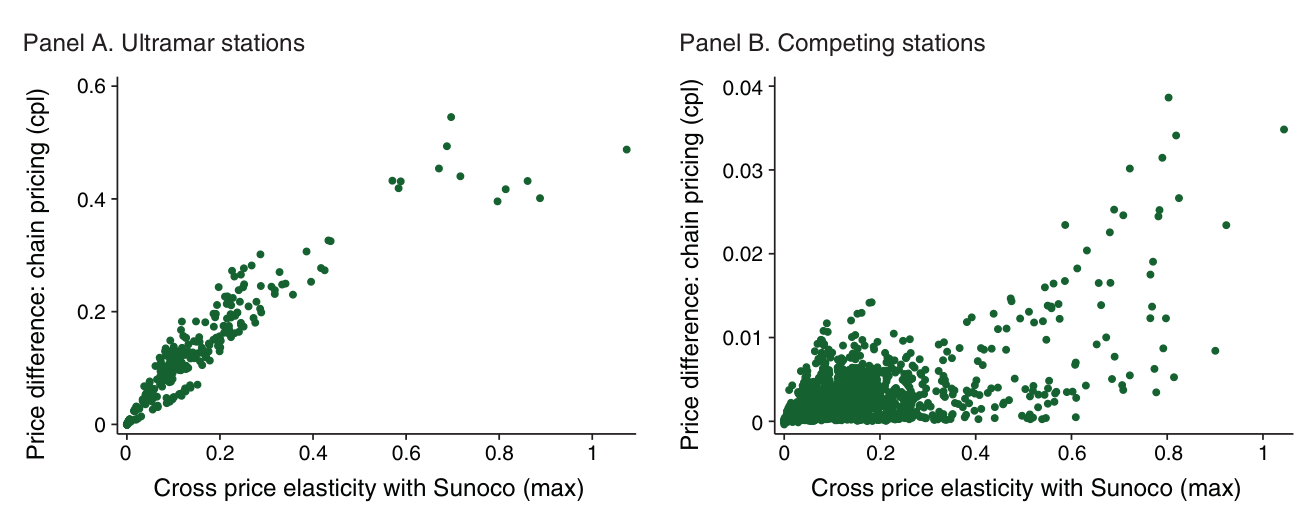
\includegraphics[width=0.92\textwidth]{figures/ch11/houde_fig4.png}
\caption{Simulated post-merger price changes (chain pricing, cpl) at Ultramar stations (panel A) and at competing
stations (panel B), plotted against each station's maximum cross-price elasticity with a Sunoco station. Note the
different vertical scales. Source: \citet{Houde2012}, Figure 4.}
\label{fig:11-houde}
\end{figure}

\Cref{fig:11-houde} shows where the price effects come from. Ultramar stations that compete closely with a Sunoco
station raise prices most, and the relation with the maximum cross elasticity is almost linear. The competitors'
responses follow the same pattern on a scale about fifteen times smaller and with more noise. Single-station owners
react more strongly to a close competitor's price increase than multi-station chains do.

\casehead{Retrospective analysis}
The difference-in-differences design follows \citet{Hastings2004}. Let $N^d_j$ indicate that station $j$ lies in
neighborhood $d$ of a Sunoco station, and let $T_t$ indicate periods from 1997 on. The indicator $S_{jt}$ marks stations
supplied by Ultramar after the merger (Ultramar, former Sunoco and Sergaz stations). The two regressions are (eqs.~(12)--(13))
\begin{align}
p_{jt} &= \gamma\, N^d_j T_t + Z_{jt}\omega + \mu_j + \tau_t + u_{jt}, \label{eq:11-houde-did}\\
p_{jt} &= \gamma_0\, N^d_j T_t S_{jt} + \gamma_1\, N^d_j T_t (1 - S_{jt}) + Z_{jt}\omega + \mu_j + \tau_t + u_{jt},
\label{eq:11-houde-did2}
\end{align}
with station fixed effects $\mu_j$, period effects $\tau_t$ and time-varying characteristics and sales volume in
$Z_{jt}$. The coefficient $\gamma$ is the average merger effect in the neighborhood, $\gamma_0$ the direct effect and
$\gamma_1$ the competitive effect. Identification requires that, absent the merger, prices in treated and control
neighborhoods would have moved in parallel. A national swap negotiated for other reasons is plausibly unrelated to
local demand shocks. The price-floor regulation introduced in 1997 must also have affected treated and control
stations alike. Standard errors are clustered by location.

\begin{table}[htbp]
\centering
\caption{Retrospective estimates of the Ultramar-Sunoco merger effect on prices (cpl)}
\label{tab:11-houde}
\begin{threeparttable}
\small
\begin{tabular}{@{}lcccccc@{}}
\toprule
\multicolumn{7}{@{}l}{\emph{Panel A. Direct and competitive effects, half-minute neighborhood (Table 11)}} \\
 & (1) & (2) & (3) & (4) & (5) & (6) \\
Sample & 95/97 & 95/97 & 95/97 & 95/97 & 95/98 & 95/98 \\
1996 price war included & Yes & Yes & No & No & No & No \\
\midrule
Merger $\times$ direct & & 0.501 & & 0.202 & & 0.211 \\
 & & (0.121) & & (0.077) & & (0.079) \\
Merger $\times$ competitive & & 0.0384 & & $-0.106$ & & 0.325 \\
 & & (0.178) & & (0.164) & & (0.169) \\
Merger (aggregate) & 0.433 & & 0.156 & & 0.229 & \\
 & (0.119) & & (0.079) & & (0.074) & \\
Observations & 5,778 & 5,778 & 5,457 & 5,457 & 7,287 & 7,287 \\
$R^2$ & 0.785 & 0.785 & 0.840 & 0.840 & 0.917 & 0.917 \\
\midrule
\multicolumn{7}{@{}l}{\emph{Panel B. Aggregate effect by neighborhood definition (Table 12)}} \\
 & \multicolumn{3}{c}{95/97, price war included} & \multicolumn{3}{c}{95/98, price war excluded} \\
\cmidrule(lr){2-4}\cmidrule(lr){5-7}
Within half a minute & \multicolumn{3}{c}{0.433 (0.119)} & \multicolumn{3}{c}{0.229 (0.074)} \\
Within one minute & \multicolumn{3}{c}{0.419 (0.110)} & \multicolumn{3}{c}{0.216 (0.064)} \\
Within 1.5 minutes & \multicolumn{3}{c}{0.290 (0.108)} & \multicolumn{3}{c}{0.223 (0.059)} \\
Common street & \multicolumn{3}{c}{0.266 (0.084)} & \multicolumn{3}{c}{0.175 (0.067)} \\
\bottomrule
\end{tabular}
\begin{tablenotes}[flushleft]
\footnotesize
\item Notes: Reproduced from \citet[Tables 11 and 12]{Houde2012}. Dependent variable: station price. The merger variable
is a Sunoco station in the neighborhood times years from 1997. The direct effect applies to post-merger Ultramar brands
(Sunoco, Sergaz and Ultramar), the competitive effect to all other stations in the neighborhood. All regressions
include location and time fixed effects and time-varying controls. Standard errors clustered by location in
parentheses. Panel B has 5,778 observations in the first column group and 7,287 in the second. The note to the paper's
Table 11 says that columns 2 to 6 exclude the 1996 price war. The text (p.~2176) and the sample sizes show that only
columns 3 to 6 do, and we follow the text.
\end{tablenotes}
\end{threeparttable}
\end{table}

\Cref{tab:11-houde} reports the estimates. Every specification finds a price increase in the treated neighborhoods,
so the market-power effect dominated any efficiency gain. The aggregate half-minute effect ranges from 0.156 to 0.433
cpl depending on the sample. Average retail margins were about 4 cpl at the time, so the merger raised margins by at
most 11 percent and prices by about 0.7 percent. In US units the increase is at most 1.75 cents per gallon. It is
smaller than the 5 cents of \citet{Hastings2004} and larger than the 1 cent of \citet{TaylorKreisleZimmerman2010}
\citep[p.~2176]{Houde2012}. The effect comes mostly from stations supplied by Ultramar, with direct
effects between 0.2 and 0.5 cpl. The competitive effect is imprecise and sometimes negative. It becomes significant
only in the sample that extends to 1998, when more stations had been rebranded. In the 1995--1997 sample with the price war, the effect declines with the size of
the neighborhood. In the 1995--1998 sample, which drops the price war and adds the rebranding period, it declines
much less (Panel B). Houde attributes the flatter profile to the rebranding periods in that sample (p.~2177).

\casehead{Comparing simulation and retrospective estimates}
The two methods agree on the main magnitude. The simulation predicts 0.38 cpl in the half-minute neighborhood, and
the aggregate retrospective estimates in \cref{tab:11-houde} range from 0.16 to 0.43 cpl. Both attribute most of the effect to the merging chain's
internalization of diversion between its old and new stations. Both find larger effects where Ultramar and Sunoco
stations competed for the same commuters.

They disagree in two ways that point to the model's weak spot. The retrospective competitive effect is larger in
one sample, and the observed effect falls more slowly with distance. The simulated effect falls from 0.388 to 0.090
cpl across the four neighborhoods, while the estimated effect falls from 0.433 to 0.266 cpl in the sample with the
price war. The logit shock makes simulated competitor responses too small, a limitation common to most differentiated
products models with idiosyncratic shocks (\cref{ch:blp}). Without the price war, the retrospective estimate (about
0.2 cpl) is below the simulated one (about 0.38 cpl, given as 0.37 in the paper's discussion). The gap may indicate
efficiencies larger than those estimated.

The retrospective design has its own weaknesses, which the simulation helps diagnose. The estimates are sensitive to
the sample, and the version with the price war may capture the end of the war in neighborhoods where Ultramar was
active, a second treatment. Controls are contaminated because distant Ultramar stations also raise prices. The
simulation also explains why two studies of the same California merger reached different answers.
\citet{Hastings2004} found price increases of about 5 cents per gallon after ARCO acquired the Thrifty chain, and
\citet{TaylorKreisleZimmerman2010} found about 1 cent with different price data. Simulated effects are very
heterogeneous across stations. Samples that omit the acquired stations or over-represent the acquirer's stations
among controls can understate the effect. Dropping Sunoco stations from the averages in \cref{tab:11-houde-sim}
would cut the direct effect by more than half \citep[pp.~2178--2179]{Houde2012}.

\casehead{Limitations and critiques}
Several assumptions deserve scrutiny. Total gasoline consumption is inelastic, so the model captures station choice
and car use but not driving more when gasoline is cheap. The price used for estimation is a single survey-day
snapshot in a market where prices change weekly, and the analysis assumes the cross-sectional price distribution is
stable within periods. Routes are deterministic shortest paths without congestion, and income is assumed independent
of workplace. The RPM assumption makes suppliers the price setters at lessee stations. The merger is small, with 12
acquired stations, which limits the power of the retrospective test. The logit shock, as Houde emphasizes, understates
the substitution between close competitors despite a large transport cost.

\casehead{Contribution}
The paper makes three contributions. It shows how to put a realistic geography into a BLP-style demand model by
treating commuting paths as consumer locations. It shows that this changes the estimates of transport costs and
markups substantially, and that the resulting markups match an external benchmark, the rack margin. It offers one of
the cleanest validations of merger simulation against a retrospective estimate of the same merger, complementing
\citet{Peters2006}, \citet{WeinbergHosken2013} and the analgesics study of \cref{sec:11-bv}. The same market reappears
in \cref{ch:collusion-evidence}, where \citet{ClarkHoude2013} study a gasoline cartel in Quebec.

\subsection{Mergers and product repositioning in music radio: Sweeting (2010)}\label{sec:11-sweeting}

\casehead{Question}
Merger analysis usually treats the set of products as fixed. In many industries a merged firm can change its products
quickly, and \citet{Sweeting2010} asks what it does with them. The question has policy weight. If merging firms
reposition their products, models with fixed products will mispredict price and welfare effects. Rivals may also lose
from a merger without synergies, which contradicts the standard Bertrand prediction that rivals gain
(\cref{sec:11-upp}).

\casehead{What theory predicts}
One-dimensional location models give stark and opposite answers. With price competition and quadratic transport
costs, two independent firms locate at the ends of the line to soften price competition
\citep{DAspremontGabszewiczThisse1979}. A merger then reduces differentiation, because the joint owner no longer needs
to soften competition between its own products. Without price competition and with a fixed audience, independent
firms cluster at the center, the minimal differentiation of \citet{Hotelling1929}. A joint owner gains nothing from
duplication and spreads its products to avoid cannibalization, a point that goes back to \citet{Steiner1952}. Reality
lies between these extremes. \citet{GandhiEtAl2008} compute equilibria of a location-then-price game and show that a
merged firm may move its products apart and toward rivals, which mitigates the price increase.

\casehead{Setting}
The 1996 Telecommunications Act relaxed local ownership caps for radio stations, and the industry consolidated
rapidly. Radio is a two-sided market. Listeners pay an implicit price by hearing commercials, and advertisers pay for
listeners. The Department of Justice reviewed radio mergers solely for their effect on advertising prices. It
required divestitures in some deals but did not consider effects on listeners or programming variety
\citep[p.~8]{Sweeting2010}. Programming changes are cheap within a format. Music licenses are blanket licenses whose
fees are a fixed share of revenue, so playlist overlap does not affect costs.

\casehead{Data}
Station characteristics, ownership histories and Arbitron audience shares come from the BIAfn MediaAccess Pro
database. Playlists come from Mediabase airplay logs for the first week (Monday to Friday) of each month from April
1998 to December 2001, for 1,094 music stations. The data contain 133,994 station-day logs. The stations belong to
seven formats (Adult Contemporary, Album Oriented Rock/Classic Rock, Contemporary Hit Radio/Top 40, Country, Oldies,
Rock, Urban) and 148 markets. In 2001 they had revenues of \$6.5 billion and an average audience of 13 million. A
station plays on average 1,367 songs by 177 artists in a five-day week, and 10,542 artists appear at least once.

The estimation sample has 740 stations in market-formats with at least two sample stations. These form 688 pairs in
the same market-format, which experience 46 changes in common ownership. Of these, 31 are mergers, that is, switches
from separate to common ownership. By type of transaction, 24 come from deals confined to one market-format and 8 from
transactions spanning more than 7 market-formats. Another 14 come from divestitures that the Department of Justice
required. Market shares convert Arbitron's average quarter-hour
shares into shares of total listening time.

\casehead{Measuring product positions}
Each station's playlist in week $w$ is a vector $a_i \in \R^{\mathcal{M}}_+$, where $\mathcal{M}$ is the set of artists
and $a_{im}$ is the share of station $i$'s songs by artist $m$. Two measures of the distance between stations $i$ and
$j$ are used. The \emph{unique-artist measure} is the average share of each station's songs by artists the other
station does not play:
\begin{equation}\label{eq:11-sw-ua}
d^{UA}_{ij} = \frac{1}{2}\Big[\sum_{m : a_{jm} = 0} a_{im} + \sum_{m : a_{im} = 0} a_{jm}\Big] \in [0, 1].
\end{equation}
The \emph{angle measure} treats each artist as a dimension and measures the angle between the two playlist vectors,
normalized by its maximum for nonnegative vectors:
\begin{equation}\label{eq:11-sw-angle}
d^{A}_{ij} = \frac{2}{\pi}\arccos\Big(\frac{a_i^{\top}a_j}{\lVert a_i\rVert\,\lVert a_j\rVert}\Big) \in [0, 1].
\end{equation}
The angle measure distinguishes stations that play the same artists in different proportions, which matters in
formats where almost every station plays the current hits. The two measures have a within-pair correlation of 0.65.
The distance between a pair $(i,j)$ and a third station $k$ in the same market-format is $\min\{d_{ik}, d_{jk}\}$.

\begin{example}[Computing the distance measures]\label{ex:11-sweeting}
Suppose there are three artists $X$, $Y$ and $Z$. Station $i$ plays them 10, 0 and 5 times, so $a_i = \big(\frac{2}{3},
0, \frac{1}{3}\big)$. Station $j$ plays $Y$ and $Z$ equally, so $a_j = \big(0, \frac{1}{2}, \frac{1}{2}\big)$. Artist
$X$ is unique to $i$ and artist $Y$ is unique to $j$, so
\begin{equation*}
d^{UA}_{ij} = \frac{1}{2}\Big[\frac{2}{3} + \frac{1}{2}\Big] = \frac{7}{12} \approx 0.583 .
\end{equation*}
For the angle, $a_i^{\top}a_j = \frac{1}{6}$, $\lVert a_i\rVert = \frac{\sqrt{5}}{3}$ and $\lVert a_j\rVert =
\frac{1}{\sqrt 2}$, so the cosine is $\frac{1}{\sqrt{10}} \approx 0.316$. The angle is 1.249 radians and
$d^{A}_{ij} = \frac{2}{\pi}\times 1.249 \approx 0.795$.
\end{example}

The cross-section already suggests the main pattern. Commonly owned pairs have an average unique-artist measure of
0.66, against 0.55 for separately owned pairs. A commonly owned station thus devotes about 20 percent more of its
playlist to artists absent from its sister station. Separately owned stations are not minimally differentiated
either. Pairs of format duopolists in the same market are more differentiated than pairs of format monopolists in
different markets of the same Census division. In Adult Contemporary, for example, the angle measures are 0.721 and
0.619 (Table 3(a)). This rules out the model without price competition, in which duopolists would cluster. The
finding that common owners differentiate more is in turn at odds with the standard two-product model with price
competition, in which a merger brings products closer together.

\casehead{Estimating equation}
The main specification is a fixed effects regression on station pairs in the same market-format
\citep[eq.~(1)]{Sweeting2010}:
\begin{equation}\label{eq:11-sw-reg}
d_{ijw} = \mathit{CO}_{ijw}\,\beta_1 + N_{ijw}\beta_2 + T_{ijw}\beta_3 + \mu_{ij} + \varepsilon_{ijw}.
\end{equation}
Here $d_{ijw}$ is the distance between stations $i$ and $j$ in week $w$, and $\mathit{CO}_{ijw}$ indicates a common
owner. The controls $N_{ijw}$ are dummies for the numbers of stations and of sample stations in the market-format,
$T_{ijw}$ are week-by-format dummies, and $\mu_{ij}$ is a pair fixed effect. The coefficient $\beta_1$ is identified by within-pair
changes in ownership, while pairs without changes help identify the time and market-structure effects. Standard
errors are clustered by market-format, which allows for correlation across pairs that share a station.

The same template is applied to other outcomes. For positioning relative to rivals, the dependent variable is the
distance between a pair and a third station. The treatment is then common ownership of the pair by a firm that does not
own the third station, with a fixed effect for each pair-third-station triplet. For variety, the dependent
variable is the log number of artists played in a market-format. For audiences, it is the pair's combined market share
with quarter-by-format effects. For prices, it is the commercial load of a station in an hour.

\casehead{Identification}
No instrument for ownership changes is available. The causal reading rests on three arguments. First, timing.
\Cref{fig:11-sweeting} shows no trend in differentiation or audiences before mergers and clear changes within six to
twelve months after them. Second, similar effects appear for small and large transactions. A deal covering dozens of
markets is unlikely to be driven by conditions in one market-format. Third, mergers and demergers produce changes of
opposite sign, although they presumably occur for different reasons.

\casehead{Main results}
\Cref{tab:11-sweeting} collects the key estimates. Common owners differentiate their stations. The angle measure
rises by 0.055 and the unique-artist share by 7.2 percentage points, 13 percent of the separately owned mean. The
effect is at least as large in market-formats with three or more observed stations, where rivals might constrain
repositioning. Common owners also move their stations closer to competitors. The distance from the pair to a third
station falls by 0.055 on the angle measure and by 6.1 percentage points on the unique-artist measure. Only the first
estimate is significant, at the 10 percent level. Variety does not rise. The number of artists in a market-format rises
by 6.9 percent only when one firm owns all observed stations, and the number of owners has no significant effect.

\begin{table}[htbp]
\centering
\caption{Ownership changes and positioning, audiences and commercial loads in radio}
\label{tab:11-sweeting}
\begin{threeparttable}
\footnotesize
\setlength{\tabcolsep}{4pt}
\begin{tabular}{@{}lcccccc@{}}
\toprule
\multicolumn{7}{@{}l}{\emph{Panel A. Differentiation between commonly owned stations (Table 4)}} \\
 & \multicolumn{2}{c}{All pairs} & \multicolumn{2}{c}{3 or more stations} & \multicolumn{2}{c}{2 stations} \\
\cmidrule(lr){2-3}\cmidrule(lr){4-5}\cmidrule(lr){6-7}
Angle measure & \multicolumn{2}{c}{0.055 (0.014)} & \multicolumn{2}{c}{0.068 (0.022)} & \multicolumn{2}{c}{0.043 (0.018)} \\
Unique-artist measure & \multicolumn{2}{c}{0.072 (0.019)} & \multicolumn{2}{c}{0.080 (0.024)} & \multicolumn{2}{c}{0.069 (0.033)} \\
Observations & \multicolumn{2}{c}{15,792} & \multicolumn{2}{c}{10,216} & \multicolumn{2}{c}{5,576} \\
\midrule
\multicolumn{7}{@{}l}{\emph{Panel B. Positioning relative to competitors and variety (Table 5)}} \\
 & \multicolumn{2}{c}{Angle distance} & \multicolumn{2}{c}{Unique-artist distance} & \multicolumn{2}{c}{Log number of artists} \\
\cmidrule(lr){2-3}\cmidrule(lr){4-5}\cmidrule(lr){6-7}
Pair has same owner & \multicolumn{2}{c}{$-0.055$ (0.033)} & \multicolumn{2}{c}{$-0.061$ (0.040)} & \multicolumn{2}{c}{} \\
All stations same owner & \multicolumn{2}{c}{} & \multicolumn{2}{c}{} & \multicolumn{2}{c}{0.069 (0.030)} \\
Number of owners & \multicolumn{2}{c}{} & \multicolumn{2}{c}{} & \multicolumn{2}{c}{0.009 (0.025)} \\
Observations & \multicolumn{2}{c}{14,475} & \multicolumn{2}{c}{14,475} & \multicolumn{2}{c}{8,942} \\
\midrule
\multicolumn{7}{@{}l}{\emph{Panel C. Market shares and competitor exit (Table 6)}} \\
 & (1) & (2) & (3) & (4) & (5) & (6) \\
Dependent variable & Log pair & Pair & Pair & Others' & Number & Sample \\
 & share & share & share & share & of rivals & rivals \\
Sample or model & All & Rivals & No rivals & Rivals & Poisson & Poisson \\
Pair has same owner & 0.031 & 0.0011 & 0.0003 & $-0.0012$ & $-0.140$ & $-0.252$ \\
 & (0.018) & (0.0003) & (0.0007) & (0.0005) & (0.076) & (0.081) \\
Observations & 3,015 & 2,911 & 2,835 & 2,911 & 2,939 & 2,939 \\
\midrule
\multicolumn{7}{@{}l}{\emph{Panel D. Commercial loads (Table 7)}} \\
 & \multicolumn{3}{c}{Commercial blocks per hour} & \multicolumn{3}{c}{Commercial minutes per hour} \\
\cmidrule(lr){2-4}\cmidrule(lr){5-7}
Owns other stations in format & \multicolumn{3}{c}{0.044 (0.044)} & \multicolumn{3}{c}{0.178 (0.193)} \\
Commonly owned competitors & \multicolumn{3}{c}{0.008 (0.062)} & \multicolumn{3}{c}{$-0.056$ (0.370)} \\
Observations & \multicolumn{3}{c}{960,634} & \multicolumn{3}{c}{960,634} \\
\bottomrule
\end{tabular}
\begin{tablenotes}[flushleft]
\footnotesize
\item Notes: Reproduced from \citet[Tables 4 to 7]{Sweeting2010}. Standard errors clustered by market-format in
parentheses, except in Panel C columns (5) and (6), where they come from a bootstrap that resamples markets. Panel A:
pair fixed effects, week-by-format and number-of-station dummies. Panel B: pair-third-station fixed effects in the first
two columns, market-format fixed effects in the third. Panel C: station-pair fixed effects and quarter-by-format dummies.
Columns (2) and (4) exclude pairs that change ownership as format duopolists. Column (3) excludes pairs that change
ownership with three or more stations in the format. Columns (2) to (4) drop the two quarters after an ownership
change. Shares are fractions of total listening. Panel D: station-format-hour fixed effects and year, month and
day-of-week interactions with format.
\end{tablenotes}
\end{threeparttable}
\end{table}

Listeners follow the playlists. Common ownership raises the pair's combined share by 3.1 percent, significant at the 10
percent level. \Cref{fig:11-sweeting}(c) shows a rise of almost 10 percent within a year, lagging the playlist changes
by a few months. The gain occurs only for pairs that face competitors. Their combined share rises by 0.0011, about 8
percent of the average pair's share, while the combined share of the other stations in the format falls by 0.0012. The
merging stations' gain is the rivals' loss. Rivals also leave the format. Common ownership reduces the number of
competing sample stations by 0.26 relative to a mean of 1.1, and the number of all competing stations by 0.36 relative
to a mean of 2.6.

Prices do not move. The average commercial load is 11.95 minutes per hour. Common owners slightly increase their loads
and stations facing common owners slightly reduce them, but neither effect is significant. These changes go the wrong
way to explain the shift in audiences, so repositioning, not price, is the channel.

\begin{figure}[htbp]
\centering
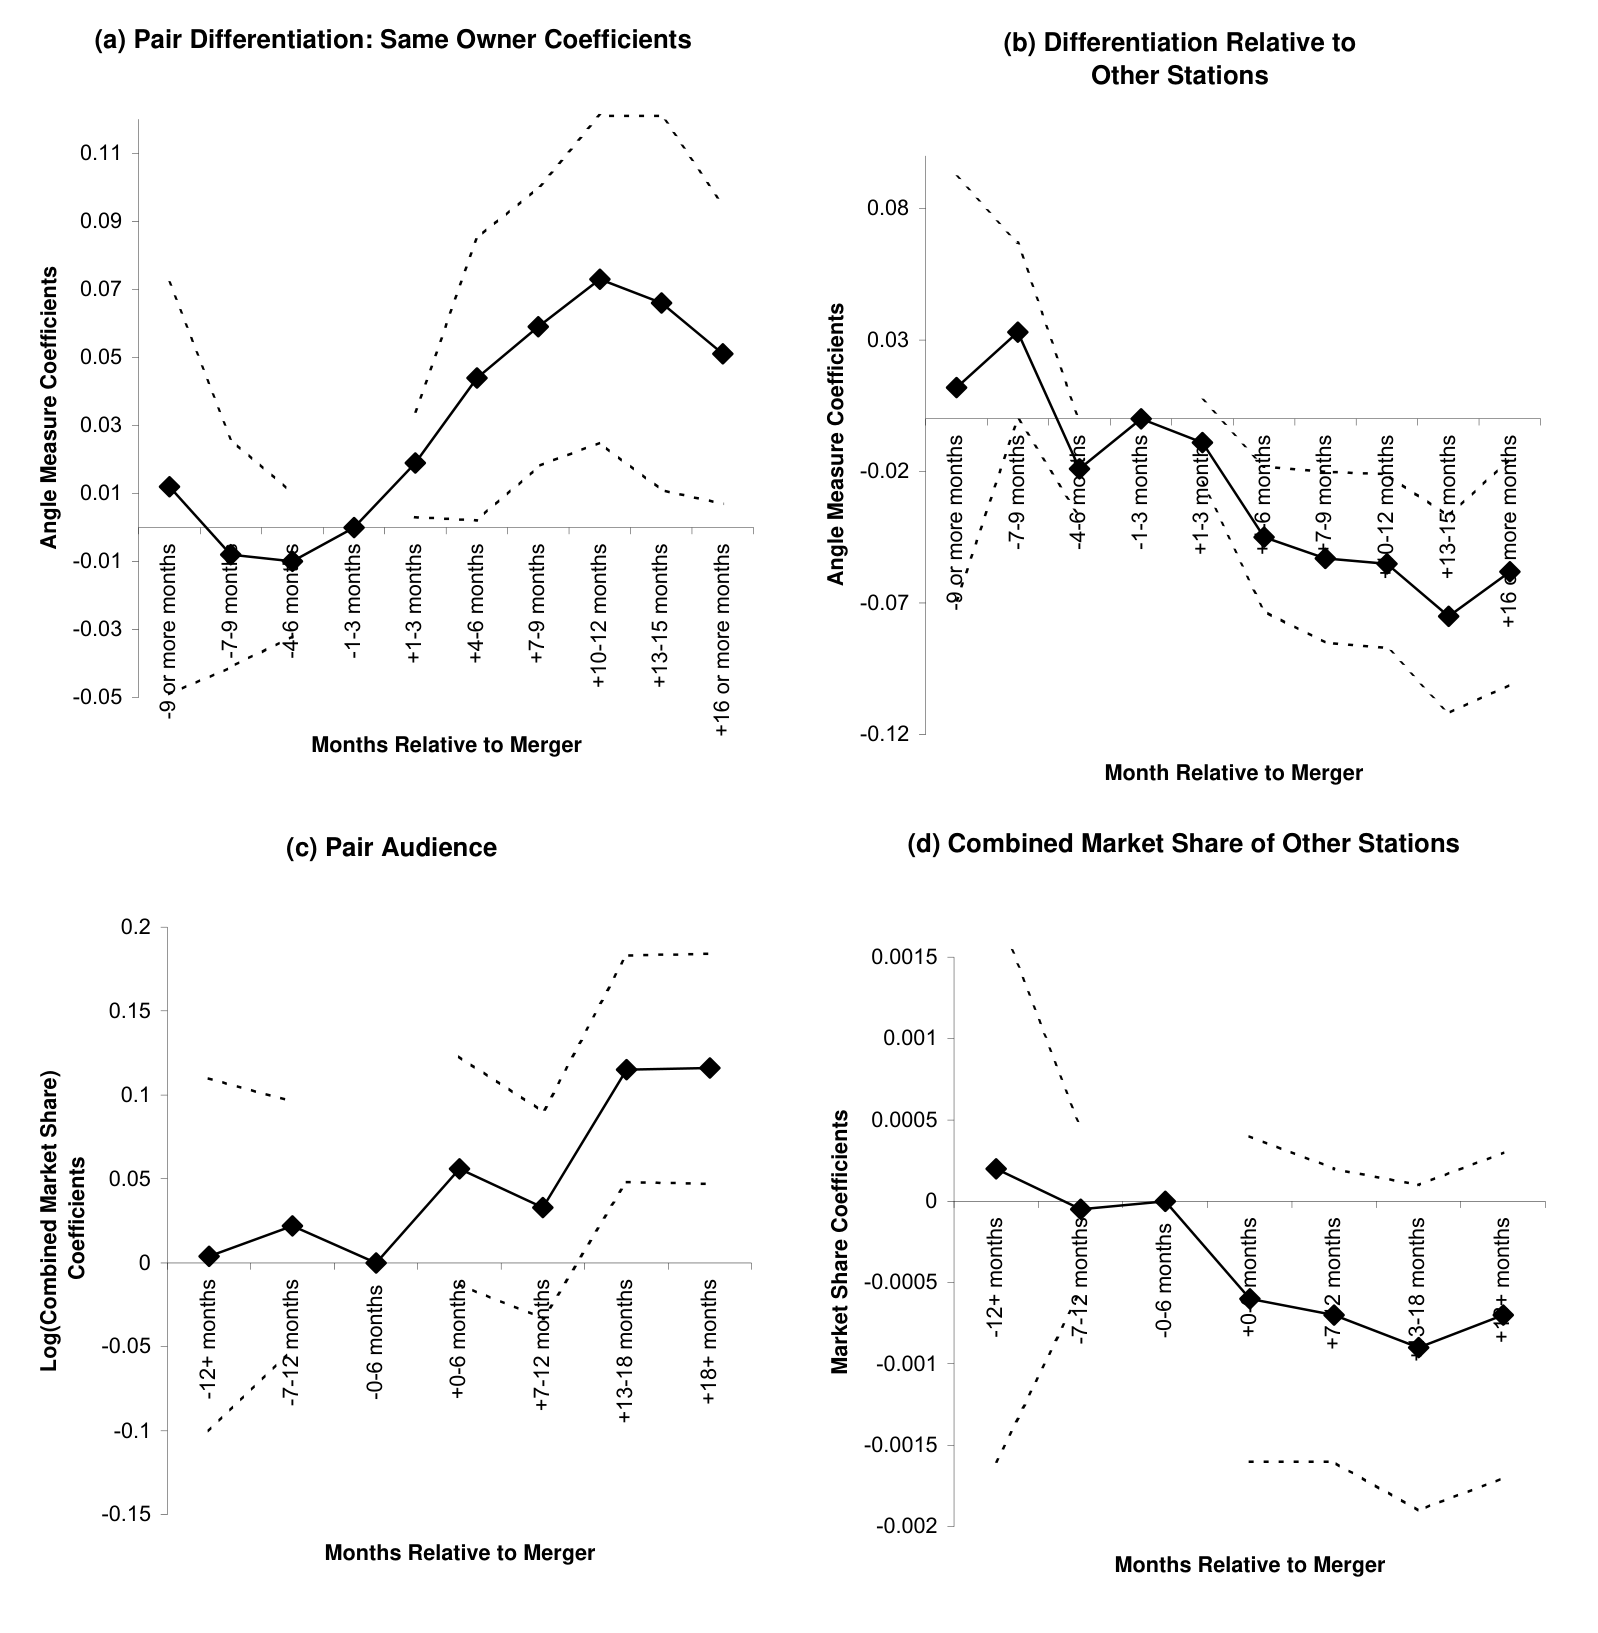
\includegraphics[width=0.84\textwidth]{figures/ch11/sweeting_fig1.png}
\caption{Timing of changes around mergers in music radio. Coefficients on dummies for time relative to the merger, with
95 percent confidence intervals (dashed). Panels (a) and (b) use the angle measure, for differentiation within the
merging pair and between the pair and other stations. Panels (c) and (d) show the log combined share of the pair and
the combined share of other stations. Pairs that ever switch from common to separate ownership are excluded. Source:
\citet{Sweeting2010}, Figure 1.}
\label{fig:11-sweeting}
\end{figure}

\casehead{Robustness}
Section~4 of the paper rules out several alternative explanations. National ownership might raise quality through
economies of scope. In a station-share regression, however, the log number of same-format stations owned nationally has
a coefficient of $-0.0003$ (0.0070), while local common ownership keeps a coefficient of 0.0554 (0.0230) (Table 8).
Changes in signal power or transmitter height do not drive the audience gains. Excluding pairs with technical changes
raises the share coefficient to 0.038 (0.022), and to 0.098 (0.017) when the two quarters after a change are dropped.
Results by format agree in sign in 19 of 21 cases (Table 9). Pairs that merge resemble other pairs before the merger on
three of four outcomes (Table 10). Results are similar for large and small transactions and for mergers and demergers
(Table 11). In data covering all formats and 281 rated markets, owning another station in the same market-format
raises a station's share by 4.6 percent (0.022). The number of owners has no effect on total format listening (Table
12).

\casehead{Interpretation}
The merged firm separates its own stations to reduce cannibalization, as a Hotelling owner without price competition
would. It also moves them toward rivals and takes their listeners. It does not use the new positions to serve
unserved tastes or to soften competition. Three implications follow for merger analysis. Models that hold products fixed will misstate the effects
of mergers, and repositioning may help explain why such models often predict post-merger prices poorly
\citep{Peters2006}. Rivals can be harmed by a merger without synergies, so their complaints do not by themselves
signal that the merger is pro-competitive. This contrasts with the logic of \cref{sec:11-cournot}. Aggregate variety
can stay constant even when the merging firms differentiate, so studies of format counts such as
\citet{BerryWaldfogel2001} see only part of the adjustment. The welfare effect of the repositioning remains open,
since moving closer to rivals transfers listeners without creating variety (\cref{ch:newgoods}).

\casehead{Limitations and contribution}
The study is descriptive and lacks an instrument for ownership. It measures positions with playlists only, ignoring
talk and personality programming. It covers relatively successful music stations in larger markets. The industry is
unusual in ways that \citet[pp.~25--26]{Sweeting2010} lists: horizontal differentiation dominates, listening is
inelastic, price competition through commercials is weak, and playlist changes do not affect costs. The paper's
contribution is a set of stylized facts that structural models of endogenous product choice should match.

Structural merger simulations with repositioning have since followed, each adapted to its industry
\citep[pp.~236--237]{AskerNocke2021}. \citet{LiEtAl2019} study airline mergers. A first-stage entry model, in which a
carrier chooses between nonstop and connecting service on a route, is attached to a nested logit demand model.
\citet{Wollmann2018} also uses a first-stage entry model, to study how a merger changes the product mix in the US
market for commercial vehicles. \citet{Fan2013} lets merging newspapers adjust their prices and three dimensions of
quality. Because the characteristics are continuous, repositioning adds first-order conditions for them to the
pricing conditions of \cref{sec:11-simframework}. \citet{MazzeoSeimVarela2018} add a product-selection stage to a
standard simulation and explore its effects in a range of simulations. \citet{DraganskaMazzeoSeim2009} study
assortment choice more broadly.

These studies agree with Sweeting that a merger can change the incentives to offer particular products, and that
allowing for repositioning changes the estimated effect on consumer welfare. They disagree on the direction of the
bias from ignoring it. Repositioning or entry by a rival adds competitive pressure, while the merged firm's exit from
a product space removes it and adds to the harm. Which force dominates depends on the industry
\citep[p.~237]{AskerNocke2021}.

\subsection{Mergers and capacity investment in the paper industry: Pesendorfer (2003)}\label{sec:11-pesendorfer}

\casehead{Question}
In industries where capacity is the main strategic variable, a merger changes the allocation of capital and the
incentives to invest. A study of short-run prices or outputs can then mismeasure the merger's effects.
\citet{Pesendorfer2003} studies the wave of 31 horizontal mergers in the US paper and paperboard industry between
August 1984 and July 1987. He models capacity investment, uses firms' investment choices before and after the wave to
infer the cost changes that mergers produced, and computes the implied welfare effects. The wave followed the 1984
revision of the Merger Guidelines, which signaled a friendlier stance toward mergers.

\casehead{The investment model}
There are $n$ firms producing a homogeneous good. Firm $i$ starts with capacity $K_i$ and chooses investment $x_i$,
which may be negative (scrapping). Capacity depreciates by the factor $\vartheta \in (0,1)$, so the post-investment
capacity is $\vartheta K_i + x_i$. Adding capacity costs $r(x_i)$, while scrapping is free. Production cost is
$C_i(\cdot)$ with marginal cost $c_i(\cdot)$. Plants run at full capacity, an assumption that fits an industry whose
utilization averaged 93 percent, so industry output is $Q = \sum_j(\vartheta K_j + x_j)$. Firms discount the future by
$\delta \in (0,1)$. Pesendorfer writes $\beta$ for the discount factor and $\delta$ for depreciation, and we rename
both to follow \cref{ch:collusion-theory}. Firm $i$'s payoff is the discounted stream of future profits from the new
capacity, minus investment cost (eq.~(1)):
\begin{equation}\label{eq:11-pes-payoff}
\Pi_i(x) = \frac{\delta}{1 - \delta}\Big[(\vartheta K_i + x_i)\,P\Big(\sum_j(\vartheta K_j + x_j)\Big) - C_i(\vartheta K_i
+ x_i)\Big] - r(x_i)\,\indic\{x_i > 0\}.
\end{equation}
The model is a one-shot investment game. Without depreciation ($\vartheta = 1$) and with linear investment cost, its
equilibrium coincides with that of a dynamic game in which all investment occurs at once.

\begin{proposition}[Equilibrium investment, after \citealp{Pesendorfer2003}, Proposition 1]\label{prop:11-pes-kt}
Let $\mathit{MR}_i = P(Q) + (\vartheta K_i + x_i)P'(Q)$ be firm $i$'s marginal revenue from capacity. Assume that an
equilibrium exists, marginal revenue decreases in own capacity, $c_i$ is nondecreasing, and $r$ is increasing and
convex. In an equilibrium, each firm's investment satisfies
\begin{equation}\label{eq:11-pes-kt}
\begin{aligned}
x_i > 0 &: \quad \frac{\delta}{1 - \delta}\big[\mathit{MR}_i - c_i\big] = r'(x_i),\\
x_i < 0 &: \quad \mathit{MR}_i - c_i = 0,\\
x_i = 0 &: \quad 0 \le \frac{\delta}{1 - \delta}\big[\mathit{MR}_i - c_i\big] \le r'(0),
\end{aligned}
\end{equation}
where $c_i$ is evaluated at $\vartheta K_i + x_i$.
\end{proposition}

\begin{proof}
Holding rivals' choices fixed, $\Pi_i$ is concave in $x_i$ on each side of zero under the stated assumptions. For
$x_i \neq 0$ its derivative is $\frac{\delta}{1-\delta}[\mathit{MR}_i - c_i] - r'(x_i)\indic\{x_i > 0\}$, and an
interior optimum sets it to zero, which gives the first two lines. At $x_i = 0$ the payoff has a kink. The left
derivative is $\frac{\delta}{1-\delta}[\mathit{MR}_i - c_i]$ and the right derivative subtracts $r'(0)$. Zero is
optimal when the left derivative is nonnegative, so scrapping does not pay, and the right derivative is nonpositive, so
investing does not pay. This gives the third line. Pesendorfer writes the three cases compactly as
$x_i\{[\mathit{MR}_i - c_i]\frac{\delta}{1-\delta} - r'(x_i)\indic\{x_i > 0\}\} = 0$ (eq.~(2)).
\end{proof}

Inverting \eqref{eq:11-pes-kt} gives marginal cost as a function of observables (Corollary 2, eq.~(3)):
\begin{equation}\label{eq:11-pes-cost}
c_i = \mathit{MR}_i - \frac{1 - \delta}{\delta}\, r'(x_i)\,\indic\{x_i > 0\} \quad (x_i \neq 0),
\qquad
c_i \in \Big[\mathit{MR}_i - \frac{1 - \delta}{\delta}\, r'(0),\; \mathit{MR}_i\Big] \quad (x_i = 0).
\end{equation}
The right-hand side depends on industry capacity and investment, the firm's own capacity and investment, demand and
the investment cost function. Marginal revenue falls with own capacity. So for a given capacity, a firm that invests
more must have a lower marginal cost. This is the inference the empirical work exploits: changes in investment after a
merger reveal changes in the merged firm's costs. Investment is measured as $x_i = K_i' - \vartheta K_i$, where $K_i'$
is next period's capacity. With $\vartheta < 1$ a firm that keeps capacity constant invests a positive amount, so the
interval case rarely arises.

\casehead{Merger analysis in a linear example}
To see what the model implies, Pesendorfer specializes it. We follow \cref{sec:11-ssr} and write the demand intercept
as $a$.

\begin{assumption}[Linear investment model]\label{ass:11-pes}
(i) Demand is $P(Q) = a - bQ$. (ii) $\frac{\delta}{1 - \delta} = \vartheta = 1$. (iii) Unmerged firms have constant
marginal cost $c$, and the merged firm has constant marginal cost $c_m$. (iv) Investment cost is linear, $r(x) = rx$.
(v) Initial capacities are at Cournot levels, $K_i = K^c \equiv \frac{a - c}{b(n + 1)}$.
\end{assumption}

Under (ii) the payoff is one period's profit minus investment cost. Before the merger, all firms hold $K^c$, the price
is $P^0 = c + \frac{a - c}{n + 1}$, each firm earns $\frac{(a - c)^2}{b(n + 1)^2}$, and no firm wants to invest or scrap.
Two firms then merge, and the merged firm $m$ holds $2K^c$.

\begin{proposition}[A profitable merger without synergies]\label{prop:11-pes-profit}
Let \cref{ass:11-pes} hold with $c_m = c$, and suppose $\frac{a - c}{2(n + 1)} \le r$. Then the post-merger game has an
equilibrium in which the merged firm scraps $\frac{K^c}{2}$ and no outsider invests. The price rises to $c +
\frac{3}{2}\,\frac{a - c}{n + 1}$, and the merging firms' joint profit rises by $\frac{1}{4b}\big(\frac{a - c}{n +
1}\big)^2 > 0$.
\end{proposition}

\begin{proof}
Use $b(n + 1)K^c = a - c$ throughout. Suppose outsiders choose $x_i = 0$ and the merged firm chooses $x_m$. Industry
output is $nK^c + x_m$. An outsider's marginal revenue minus cost is
\begin{equation*}
\mathit{MR}_i - c = a - c - b(nK^c + x_m) - bK^c = (a - c) - b(n + 1)K^c - b\,x_m = -b\,x_m .
\end{equation*}
The merged firm's is
\begin{equation*}
\mathit{MR}_m - c = a - c - b(nK^c + x_m) - b(2K^c + x_m) = -\frac{a - c}{n + 1} - 2b\,x_m .
\end{equation*}
This is negative at $x_m = 0$, so the merged firm scraps until $\mathit{MR}_m = c$:
\begin{equation*}
x_m = -\frac{a - c}{2b(n + 1)} = -\frac{K^c}{2}.
\end{equation*}
Its payoff is concave, and investing is never optimal because $\mathit{MR}_m - c - r < 0$ for $x_m \ge 0$. Given
$x_m$, each outsider has $\mathit{MR}_i - c = \frac{a - c}{2(n + 1)} \ge 0$, so scrapping does not pay. Investing
does not pay if this gain is at most $r$, which is the stated condition. So $x_i = 0$ is a best response.

Industry output is $\big(n - \frac{1}{2}\big)K^c$, and the margin is
\begin{equation*}
P - c = (a - c) - \Big(n - \frac{1}{2}\Big)\frac{a - c}{n + 1} = \frac{3}{2}\,\frac{a - c}{n + 1}.
\end{equation*}
The merged firm sells $\frac{3}{2}K^c$, so its profit is $\frac{3}{2}\frac{a - c}{n + 1}\times\frac{3}{2}\frac{a - c}{b(n
+ 1)} = \frac{9}{4b}\big(\frac{a - c}{n + 1}\big)^2$. Before the merger the two firms earned $\frac{2}{b}\big(\frac{a -
c}{n + 1}\big)^2$. The difference is $\frac{1}{4b}\big(\frac{a - c}{n + 1}\big)^2$.
\end{proof}

\citet[Remark 3]{Pesendorfer2003} states the result under the condition $n + 1 > \frac{a - c}{r}$, which implies the
weaker condition used above. The mechanism is the asymmetry between expanding and contracting capacity. The merged firm
can withdraw capacity at no cost, while outsiders would have to pay $r$ per unit to fill the gap. If $r = 0$, outsiders
expand freely, every firm sets $\mathit{MR} = c$, and the post-merger outcome is Cournot with $n - 1$ firms. A
two-firm merger is then unprofitable for $n \ge 3$ (\cref{prop:11-ssr}). For any $r > 0$, however, a profitable merger
exists once $n$ is large enough \citep[p.~7, n.~6]{Pesendorfer2003}.

\begin{example}[Investment makes the merger profitable]\label{ex:11-pes}
Let $a = 10$, $b = 1$, $c = 2$, $n = 4$ and $r = 1$. Cournot capacities are $K^c = 1.6$, the price is $P^0 = 3.6$ and
each firm earns 2.56. After a merger of two firms, the merged firm scraps 0.8 units, outsiders' marginal gain from
investing is $0.8 < r$, and the price rises to 4.4. The merged firm earns $2.4 \times 2.4 = 5.76$, a gain of 0.64 over
the combined 5.12. Pesendorfer's sufficient condition would require $r > 1.6$, so the example lies in the region
covered only by the weaker condition. With costless expansion the outcome would be Cournot with three firms, a price of
4.0 and a merged profit of 4.0, a loss of 1.12. Costly expansion makes the merger profitable precisely because rivals
do not replace the withdrawn capacity, so consumers face a higher price than in the Cournot benchmark.
\end{example}

The example shows a general feature. The post-merger margin is $\frac{3}{2}\frac{a - c}{n + 1}$, while the Cournot
margin with $n - 1$ firms is $\frac{a - c}{n}$. The first is larger whenever $n > 2$. Pesendorfer's three remaining
remarks describe what investment reveals about costs and welfare.

\begin{proposition}[Investment and merger cost savings, Remarks 4 to 6]\label{prop:11-pes-remarks}
Let \cref{ass:11-pes} hold.
\begin{enumerate}[label=(\alph*)]
  \item If the merged firm does not change its capacity after the merger ($x_m = 0$), then no outsider does either, and
  $2c - P^0 - r \le c_m \le 2c - P^0$. In particular $c_m < c$.
  \item If $c_m = c$, industry capacity falls and the merger reduces total welfare.
  \item If $x_m = 0$, consumer surplus is unchanged and total welfare rises.
\end{enumerate}
\end{proposition}

\begin{proof}
(a) With $x_m = 0$ and symmetric outsiders, an outsider's marginal gain is $-b(n - 1)x_i$. A positive $x_i$ would
require this to equal $r > 0$, and a negative $x_i$ would require it to equal zero, so $x_i = 0$. The merged firm's
marginal revenue at $x_m = 0$ is $a - b(n + 2)K^c = P^0 - 2(P^0 - c) = 2c - P^0$. Zero investment requires $0 \le
\mathit{MR}_m - c_m \le r$, which is the stated band. Since $P^0 > c$, $c_m \le 2c - P^0 < c$.

(b) Suppose instead that total investment $X = \sum_j x_j$ is positive. An outsider's marginal gain is $-b(X + x_i)$,
which cannot equal $r > 0$ when $x_i > 0$ and $X > 0$, so $x_i \le 0$. The merged firm's is $-\frac{a - c}{n + 1} -
b(X + x_m)$, which is negative when $x_m > 0$ and $X > 0$, so $x_m \le 0$. Then $X \le 0$, a contradiction. If $X = 0$,
the merged firm's marginal gain at any $x_m \ge 0$ is negative, so it scraps. Outsiders would then have to invest, but
an outsider with $x_i > 0$ has marginal gain $-b\,x_i < 0 < r$. Hence $X < 0$. Output falls below the pre-merger level, at which price exceeds the common marginal cost,
so total surplus falls.

(c) By part (a), output is unchanged, so price and consumer surplus are unchanged. Producer surplus rises because the
merged firm produces the same capacity at $c_m < c$.
\end{proof}

Part (a) connects the investment model to \cref{prop:11-synergy}. If nobody adjusts capacity, output and price are
unchanged, so the merger must be at least price-neutral. The merged firm's cost must then lie at or below the
price-neutral level $2c - P^0$ of the Cournot analysis. In \cref{ex:11-pes}, $2c - P^0 = 0.4$, an 80 percent cost
reduction. Unchanged investment after a merger thus reveals large savings. Consumer surplus and producer surplus
are defined as usual (eqs.~(4)--(5)):
\begin{equation}\label{eq:11-pes-welfare}
\mathit{CS} = \int_0^Q P(z)\,\dd z - Q\,P(Q), \qquad
\mathit{PS} = \sum_i\big[K_iP(Q) - C_i(K_i) - r(x_i)\indic\{x_i > 0\}\big].
\end{equation}

\casehead{Data}
Plant-level annual capacities by product for 1978--1992 come from Lockwood's Directory of the Paper and Allied Trades,
supplemented by Census price data. Products fall into nine categories: newsprint, packaging papers, groundwood printing,
coated papers, uncoated papers, other papers, tissue, linerboard and boxboard. Products within a category are largely
homogeneous, and about 80 percent of capacity is in plants producing a single category, so each category is treated as
a separate market. Newsprint is dropped because about half of US newsprint capacity is imported from Canada. The
geographic market is the United States, with exports of about 15 percent of production and imports of about 12 percent
in 1991.

Table~1 of the paper summarizes the industry. The average number of firms per category fell from 70.6 in 1978 to 60.4
in 1992. The five largest firms held on average 56.1 percent of capacity in 1992, from 41 percent in newsprint to 75
percent in tissue. Capacity grew by about 20 percent over the period, at about 0.7 percent a year before 1987 and 2.4
percent after. About 40 percent of capacity expansions at existing firms came through horizontal acquisitions, and about
40 percent of the 819 plants were involved in at least one merger. The 1984--1987 wave included Champion
International's acquisition of St.~Regis (\$1.8 billion), Jefferson Smurfit's of Container Corporation (\$1.2 billion)
and International Paper's of Hammermill (\$1.1 billion). The Federal Trade Commission blocked James River's acquisition
of Barlow Rand in February 1988. Every category had at least one merger in the wave.

\casehead{Descriptive evidence}
Merged firms' outcomes vary widely. Table~3 regresses the merged firm's share, relative to its share at the merger, on
time since the merger and its square. In the pooled data the coefficients are $-3.66$ ($t = 5.9$) and $0.35$ ($t =
3.0$), with $R^2 = 0.04$ and 1,112 observations. The share falls to about 90 percent of its initial level after about five
years and then recovers. About two-thirds of acquirers lose share and one-third gain. Probit models of annual investment
decisions on 9,352 firm-years show that a merger raises the probability of changing capacity. The coefficient on the
relative size of the acquired firm is 0.7589 ($t = 3.5$), and the coefficient on an acquisition two to five years
earlier is 0.6004 ($t = 2.4$). The effect works mostly through scrapping, with coefficients of 0.8017 ($t = 2.9$) and 0.7027 ($t = 2.2$), while
the effects on investing are positive but insignificant (Table 4). About 24 percent of firms change capacity in a given
year, three-quarters of them upward.

\casehead{Estimation}
Costs are estimated in two steps for three-year windows before and after the wave, since new capacity takes two to
three years to become usable. The wave is assumed to have been unanticipated when the earlier investments were made.
The first step estimates constant-elasticity inverse demand for each category,
\begin{equation}\label{eq:11-pes-demand}
\ln P_t = \alpha_x x_t + \gamma \ln Q_t + u_t, \qquad u_t = \varrho\, u_{t-1} + v_t, \quad |\varrho| < 1,
\end{equation}
with gross domestic product as the demand shifter $x_t$ and wages of paper workers as the instrument for output. The
second step computes each firm's marginal revenue $\widehat{\mathit{MR}}_i = \hat P(Q) + \hat P'(Q)K_i$ and recovers its
marginal cost from \eqref{eq:11-pes-cost}. The discount factor is 0.95 per year. The investment cost has a linear and
a quadratic term calibrated to reported costs of investment projects in the trade press. The base specification sets
the depreciation factor to 0.999 with linear coefficient 26.50 and quadratic coefficient 0.005, and four alternatives
vary these values.

\casehead{Cost results}
Acquiring firms have lower estimated marginal costs than unmerged firms before the wave, and the gap widens after it.
In groundwood printing, for instance, the median difference between acquiring and unmerged firms grows from \$4.39 to
\$8.01 per ton, and the mean difference from \$6.97 to \$12.87 (Table 5A). The median gap widens in all eight categories
and the mean gap in seven, the exception being boxboard. To separate merger effects from industry-wide cost changes,
Pesendorfer assigns each cost estimate its percentile in the distribution of unmerged firms' costs, before and after
the wave. \Cref{fig:11-pesendorfer} shows the result. About 90 percent of acquiring firms move to lower percentiles,
and about 10 percent do not. The Champion-St.~Regis merger is an example of expected synergies that did not
materialize.

\begin{figure}[htbp]
\centering
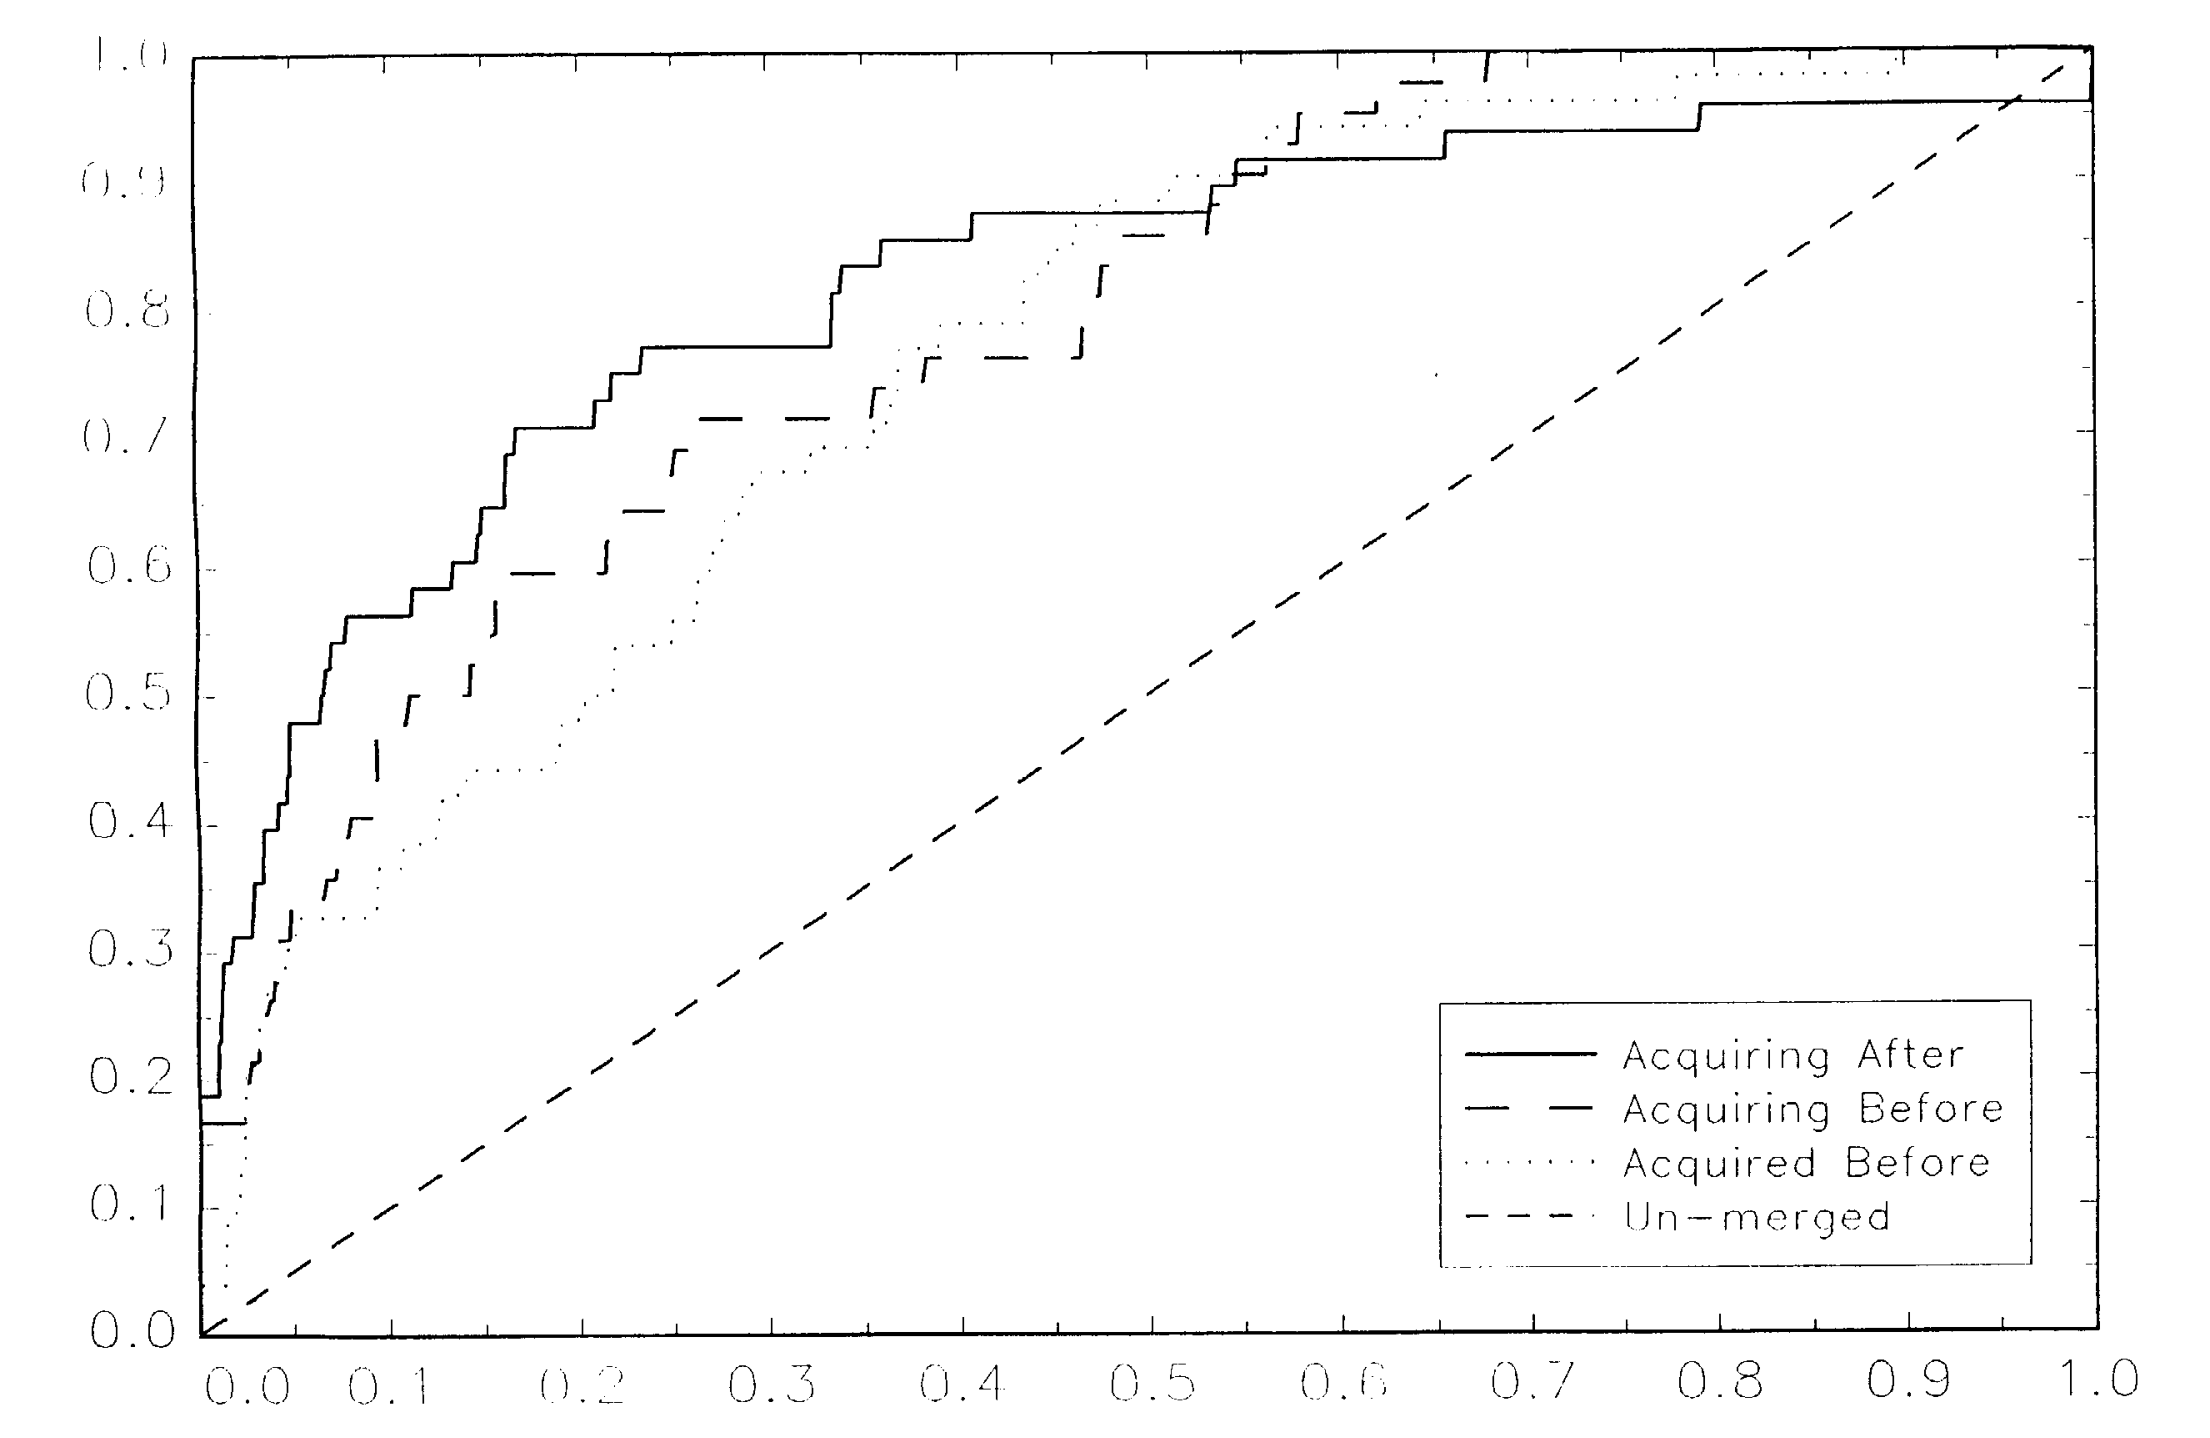
\includegraphics[width=0.72\textwidth]{figures/ch11/pesendorfer_fig2.png}
\caption{Distribution of estimated marginal costs, pooled across paper categories. Each firm's cost is expressed as
its percentile in the cost distribution of unmerged firms (horizontal axis). The curves are cumulative distribution
functions (vertical axis) for acquiring firms after and before the merger wave and for acquired firms before it. The dashed diagonal
is the distribution of unmerged firms. Curves farther above the diagonal indicate lower relative costs. The image is
rotated from the working-paper version. Source: \citet{Pesendorfer2003}, Figure 2.}
\label{fig:11-pesendorfer}
\end{figure}

\casehead{Welfare}
For the counterfactual without mergers, each merging firm's cost is projected to its post-wave level using its
percentile in the unmerged distribution. The merged firm is replaced by its components with these costs, the
investment equilibrium of \eqref{eq:11-pes-kt} is recomputed, and the changes in consumer and producer surplus follow
from \eqref{eq:11-pes-welfare}. Standard errors come from repeated draws of the projection error. \Cref{tab:11-pesendorfer}
reproduces the base specification.

\begin{table}[htbp]
\centering
\caption{Welfare effects of the 1984--1987 paper merger wave (thousands of 1986 dollars)}
\label{tab:11-pesendorfer}
\begin{threeparttable}
\small
\begin{tabular}{@{}lrrrrr@{}}
\toprule
Category & \makecell[r]{Total\\ welfare} & \makecell[r]{Consumer\\ surplus} & \makecell[r]{Producer\\ surplus} &
\makecell[r]{Merged\\ firms} & \makecell[r]{Unmerged\\ firms} \\
\midrule
Packaging papers & 61,440 & 9,499 & 51,940 & 57,090 & $-5{,}149$ \\
 & (14,635) & (6,174) & (9,145) & (12,135) & (3,494) \\
Groundwood printing & 1,736 & 3,132 & $-1{,}395$ & 419 & $-1{,}815$ \\
 & (12,187) & (6,380) & (6,393) & (9,207) & (3,213) \\
Coated papers & 9,617 & 10,604 & $-987$ & 5,708 & $-6{,}695$ \\
 & (11,036) & (11,241) & (3,950) & (7,321) & (7,118) \\
Uncoated papers & 16,826 & 21,277 & $-4{,}451$ & 9,747 & $-14{,}198$ \\
 & (21,463) & (10,197) & (13,863) & (18,991) & (7,234) \\
Other papers & 31,166 & 4,888 & 26,278 & 28,832 & $-2{,}554$ \\
 & (4,094) & (1,713) & (2,479) & (3,439) & (1,036) \\
Tissue & 298,692 & 96,089 & 202,604 & 242,905 & $-40{,}301$ \\
 & (14,676) & (7,950) & (6,815) & (11,952) & (5,240) \\
Boxboard & 412 & $-22{,}098$ & 22,510 & 11,832 & 10,679 \\
 & (16,381) & (8,594) & (8,412) & (12,233) & (4,235) \\
Linerboard & 163,587 & 90,203 & 73,384 & 112,771 & $-39{,}386$ \\
 & (82,962) & (64,079) & (52,942) & (60,261) & (28,788) \\
\midrule
Sum over categories & 583,476 & 213,594 & 369,883 & 469,304 & $-99{,}419$ \\
Range over five specifications & 454,483 to & $-58{,}555$ to & 244,271 to & & \\
 & 583,476 & 213,594 & 527,289 & & \\
\bottomrule
\end{tabular}
\begin{tablenotes}[flushleft]
\footnotesize
\item Notes: Reproduced from \citet[Table 6, specification (1): depreciation factor 0.999, linear investment-cost
coefficient 26.50, quadratic 0.005]{Pesendorfer2003}, working-paper version. Standard deviations from the projection
error in parentheses. The table reports categories only. The sums and ranges are our calculations from all five
columns of the table. The other specifications use (0.950, 26.50, 0.005), (0.999, 36.50, 0.007), (0.999, 53.00, 0)
and (0.999, 0, 0.010).
\end{tablenotes}
\end{threeparttable}
\end{table}

Summing over categories, the wave raised total welfare by \$583.5 million in the base specification, with \$213.6
million going to consumers and \$369.9 million to producers. The sums across the five specifications range from \$454
million to \$583 million for total welfare and from \$244 million to \$527 million for producer surplus. The text of the
paper gives a consumer range of \$58 million to \$210 million, while the table's columns sum to between $-\$58.6$ million
and \$213.6 million.
Merged firms gained \$469.3 million and unmerged firms lost \$99.4 million.
The text reports the merged firms' gain as \$468.3 million in two places and \$469.3 million in a third. The table
sums to the latter. The paper describes the packaging-paper figure as an increase in annual total welfare
\citep[p.~19]{Pesendorfer2003}, so the totals are best read as annual flows. Gains to merged firms are positive in every
category in the base specification. Pesendorfer states that these gains are positive in six of eight categories, with
insignificant losses in some specifications for groundwood printing and boxboard \citep[p.~21]{Pesendorfer2003}. His
Table 6 also shows insignificant losses in one specification each for uncoated papers ($-703$ thousand) and
linerboard ($-26{,}638$ thousand). Only packaging, coated, other papers and tissue show gains in every specification.
Pesendorfer reads the positive gains as support for the model, since profitability was not imposed in estimation.

\casehead{Interpretation and critiques}
The welfare gains rest on estimated cost reductions, and their distribution deserves attention. Tissue alone accounts
for 51 percent of the total welfare gain and 52 percent of the merged firms' gain. The tissue category had a single
acquiring firm (Table 2), whose estimated cost advantage over the median unmerged firm grew from \$5.71 to \$143.04 per
ton (Table 5A). The headline number thus depends heavily on one firm's inferred cost decline. More generally, marginal
costs are residuals of a first-order condition, so any misspecification of demand, of the investment cost function or
of conduct is loaded into the cost estimates. The model is static and assumes the wave was unanticipated. It treats
each category as a national homogeneous-good market with full utilization. The percentile projection assumes that, absent
mergers, each firm would have kept its relative position. Mergers are taken as given, so firms that merged may differ
from others in ways that also explain later cost changes.

\casehead{Contribution}
The paper shows that the investment channel can reverse two conclusions of static Cournot theory. Mergers without
synergies can be profitable, and the price effect of a merger depends on rivals' ability to add capacity. It also
shows how revealed investment behavior can identify merger efficiencies, an idea that complements the retrospective
price studies of \cref{sec:11-retro}. Dynamic models of mergers with investment, such as \citet{BerryPakes1993} and
\citet{Gowrisankaran1999}, develop the same concerns with richer state spaces.

\section{Merger policy with merger choice}\label{sec:11-policy}

The standard approach to merger review evaluates each proposed merger on its own. An authority with a consumer surplus
standard approves a merger if and only if it does not lower consumer surplus. This rule ignores that firms choose which
merger to propose, while the authority sees only the proposal. \citet{NockeWhinston2013} show that the choice changes
the optimal policy. If firms prefer larger mergers for reasons unrelated to consumers, the authority should hold larger
mergers to a stricter standard. \citet{Lyons2003} first identified the problem. \citet{ArmstrongVickers2010} analyze
delegated choice among projects that are ex ante identical. \citet{NockeWhinston2010} show that a myopic consumer
surplus standard is optimal in a dynamic setting when possible mergers are disjoint, that is, involve different firms.
We follow the working-paper version of \citet{NockeWhinston2013}, whose numbering may differ from the published
article.

\subsection{The model}\label{sec:11-nw-model}

Firms $i \in \mathcal{N} = \{0, 1, \dots, N\}$ produce a homogeneous good with constant marginal costs $c_i$ and
compete in quantities. Inverse demand $P(Q)$ satisfies, for all $Q$ with $P(Q) > 0$,
\begin{equation}\label{eq:11-nw-ass}
P'(Q) < 0, \qquad P'(Q) + QP''(Q) < 0, \qquad \lim_{Q \to \infty}P(Q) = 0 .
\end{equation}
These conditions imply a unique Cournot equilibrium that is stable: each best response $b_i(Q_{-i})$ has slope in
$(-1, 0)$, so if some firms want to produce less, industry output falls. All firms are active, and the pre-merger
outputs satisfy $P(Q^0) + P'(Q^0)q_i^0 = c_i$. Write $P^0 = P(Q^0)$, $s_i^0 = \frac{q_i^0}{Q^0}$ and $\pi_i^0 = (P^0 -
c_i)q_i^0$.

Firm 0, the acquirer, can merge with one target $k \in \mathcal{K} = \{1, \dots, K\}$. Targets are ordered by decreasing
cost, $c_1 > c_2 > \dots > c_K$, so a higher $k$ means a larger pre-merger share. We call merger $k$ \emph{larger}
than merger $j$ if $k > j$. The change in the naively computed Herfindahl index, which keeps all shares fixed and adds
the merging shares, is
\begin{equation}\label{eq:11-nw-hhi}
\Delta\HHI^{naive}(M_k) = (s_0^0 + s_k^0)^2 - (s_0^0)^2 - (s_k^0)^2 = 2 s_0^0 s_k^0 ,
\end{equation}
the formula of \eqref{eq:11-dhhi}. A larger merger thus has a larger naive increase in concentration.

Merger $k$ is feasible with probability $\phi_k \in (0, 1]$, independently across targets. If feasible, it yields a
post-merger marginal cost $\bar c_k$ drawn from a distribution $G_k$ with support $[c^L, c_k^H]$ and no mass points. A
feasible merger is $M_k = (k, \bar c_k)$. After merger $M_k$ the outputs solve $P(Q(M_k)) + P'(Q(M_k))q_i(M_k) = c_i$
for nonmerging firms and the same condition with $\bar c_k$ for the merged firm. All firms remain active. The changes in
consumer surplus and in the merging parties' joint (bilateral) profit are
\begin{equation}\label{eq:11-nw-changes}
\Delta \mathit{CS}(M_k) = \int_0^{Q(M_k)}P(z)\,\dd z - P(Q(M_k))Q(M_k) - \mathit{CS}^0,
\qquad
\Delta\Pi(M_k) = \pi_k(M_k) - (\pi_0^0 + \pi_k^0).
\end{equation}
A merger is \emph{CS-neutral} if $\Delta\mathit{CS} = 0$, CS-increasing if it is positive, CS-decreasing if it is
negative, and CS-nondecreasing if it is not CS-decreasing. The status quo $M_0$ gives zero changes. Let $\mathcal{F}$
be the realized set of feasible mergers, including $M_0$.

The timing has four stages. The authority commits to an approval set $\mathcal{A} = \{M_k : \bar c_k \in
\mathcal{A}_k\} \cup \{M_0\}$, where each $\mathcal{A}_k \subseteq [c^L, c_k^H]$ is a union of closed intervals. Nature
draws $\mathcal{F}$. Firms bargain over which merger to propose. The authority approves the proposal if it lies in
$\mathcal{A}$, and firms compete. The authority observes every characteristic of the proposed merger but nothing about
mergers that are not proposed, and only one merger can be proposed.

Bargaining follows the offer game of \citet{Segal1999}. Firm 0 makes a take-it-or-leave-it offer of a price $t_k$ to one
target. Setting $t_k$ to make the target indifferent, firm 0 captures the whole bilateral gain $\Delta\Pi(M_k)$. The
proposed merger is therefore
\begin{equation}\label{eq:11-nw-proposal}
M^*(\mathcal{F}, \mathcal{A}) =
\begin{cases}
\argmax_{M_k \in \mathcal{F} \cap \mathcal{A}} \Delta\Pi(M_k) & \text{if } \max_{M_k \in \mathcal{F} \cap \mathcal{A}}
\Delta\Pi(M_k) > 0,\\
M_0 & \text{otherwise.}
\end{cases}
\end{equation}
The authority chooses $\mathcal{A}$ to maximize $\E_{\mathcal{F}}\big[\Delta\mathit{CS}(M^*(\mathcal{F}, \mathcal{A}))
\big]$. One assumption avoids trivial cases. Each merger's cost support contains CS-increasing and CS-nonincreasing
outcomes, $\Delta\mathit{CS}(k, c_k^H) \le 0 < \Delta\mathit{CS}(k, c^L)$.

\subsection{Three lemmas on the shape of merger outcomes}\label{sec:11-nw-lemmas}

Because the good is homogeneous, a merger raises consumer surplus if and only if it raises industry output. The first
lemma characterizes CS-neutral mergers. It restates \cref{prop:11-synergy,cor:11-neutral-profit} in the notation of
this section.

\begin{lemma}[CS-neutral mergers]\label{lem:11-nw1}
Suppose merger $M_k$ is CS-neutral. Then (i) no nonmerging firm changes its output, and the merged firm produces
$q_0^0 + q_k^0$. (ii) The merged firm's margin equals the sum of the partners' margins,
\begin{equation}\label{eq:11-nw-neutral}
P^0 - \bar c_k = (P^0 - c_0) + (P^0 - c_k), \quad\text{so}\quad \bar c_k = \hat c_k \equiv c_k - (P^0 - c_0) <
\min\{c_0, c_k\}.
\end{equation}
(iii) The merger is profitable, $\Delta\Pi(M_k) > 0$. (iv) It raises aggregate profit.
\end{lemma}

\begin{proof}
A CS-neutral merger leaves $Q$, and hence $P$ and $P'$, unchanged. Each nonmerging firm's first-order condition then
gives the same output, and the merged firm produces the rest, $q_0^0 + q_k^0$. Its first-order condition is $P^0 +
P'(Q^0)(q_0^0 + q_k^0) = \bar c_k$. Adding the partners' pre-merger conditions gives $2P^0 + P'(Q^0)(q_0^0 + q_k^0) =
c_0 + c_k$. Subtracting the first equation from the second gives $P^0 = c_0 + c_k - \bar c_k$, which is
\eqref{eq:11-nw-neutral}. Part (iii) is \cref{cor:11-neutral-profit}: the merged profit exceeds $\pi_0^0 + \pi_k^0$ by
$(P^0 - c_0)q_k^0 + (P^0 - c_k)q_0^0 > 0$. For (iv), nonmerging firms' profits are unchanged because their prices and
outputs are unchanged.
\end{proof}

\begin{lemma}[Lower post-merger cost]\label{lem:11-nw2}
Conditional on merger $M_k$, a lower $\bar c_k$ raises industry output, consumer surplus and the merged firm's profit.
\end{lemma}

\begin{proof}
Summing the $N$ post-merger first-order conditions gives $NP(Q) + QP'(Q) = \bar c_k + \sum_{i \neq 0, k}c_i$. The
left side decreases in $Q$, because its derivative is $(N + 1)P' + QP'' < 0$ by \eqref{eq:11-nw-ass}. A lower
$\bar c_k$ lowers the right side, so $Q$ rises, and so does consumer surplus. For the profit, define the
\emph{cumulative best reply} $\tilde q(Q; c) = -\frac{P(Q) - c}{P'(Q)}$, the output at which a firm with cost $c$
satisfies its first-order condition when industry output is $Q$. Its derivative in $Q$ is
\begin{equation*}
\frac{\partial\tilde q}{\partial Q} = -1 + \frac{(P - c)P''}{(P')^2} = -1 - \frac{\tilde q\,P''}{P'} =
-\frac{P' + \tilde q P''}{P'} < 0,
\end{equation*}
using $P - c = -P'\tilde q$ and $P' + qP'' < 0$ for $q \le Q$. Nonmerging outputs $\tilde q(Q; c_i)$ therefore fall
when $\bar c_k$ falls. The merged firm's profit is $\max_q[P(Q_{-m} + q) - \bar c_k]q$, where $Q_{-m}$ is rivals'
output. By the envelope theorem its derivative in $\bar c_k$ is $-q_m + q_m P'(Q)\frac{dQ_{-m}}{d\bar c_k}$. Both terms
are negative, since $P' < 0$ and rivals' output rises with $\bar c_k$.
\end{proof}

Lemma~\ref{lem:11-nw2} implies that merger $M_k$ is CS-increasing if $\bar c_k < \hat c_k$ and CS-decreasing if
$\bar c_k > \hat c_k$. The third lemma is the key to the paper. It shows that firms' proposal incentives are biased
toward larger mergers.

\begin{lemma}[Firms prefer larger mergers]\label{lem:11-nw3}
Suppose mergers $M_j$ and $M_k$, with $k > j \ge 1$, induce the same nonnegative change in consumer surplus. Then the
larger merger induces a larger gain in bilateral profit: $\Delta\Pi(M_k) > \Delta\Pi(M_j) > 0$.
\end{lemma}

\begin{proof}
Each firm's first-order condition gives $P - c_i = -P' q_i$, so its profit is
\begin{equation}\label{eq:11-nw-profit}
\pi_i = (P - c_i)q_i = -P'(Q)\,\big[\tilde q(Q; c_i)\big]^2 .
\end{equation}
Equal consumer surplus means equal industry output $\bar Q$. Industry output depends only on the sum of active
firms' costs, by the summed first-order condition in the proof of Lemma~\ref{lem:11-nw2}. So both mergers reduce the
partners' combined cost by the same amount, $\gamma \equiv c_k - \bar c_k = c_j - \bar c_j$. Since $\frac{\partial\tilde
q}{\partial c} = \frac{1}{P'}$, the difference in the merged firms' profits is
\begin{align}
\pi_k(M_k) - \pi_j(M_j)
&= -P'(\bar Q)\Big\{\big[\tilde q(\bar Q; c_k - \gamma)\big]^2 - \big[\tilde q(\bar Q; c_j - \gamma)\big]^2\Big\}
\notag\\
&= -P'(\bar Q)\int_{c_j}^{c_k} 2\,\tilde q(\bar Q; c - \gamma)\,\frac{1}{P'(\bar Q)}\,\dd c
= 2\int_{c_k}^{c_j}\tilde q(\bar Q; c - \gamma)\,\dd c . \label{eq:11-nw-diff1}
\end{align}
The same steps applied to pre-merger profits give
\begin{equation}\label{eq:11-nw-diff0}
\pi_k^0 - \pi_j^0 = 2\int_{c_k}^{c_j}\tilde q(Q^0; c)\,\dd c .
\end{equation}
Now consider, for any $c \in [c_k, c_j]$, a merger of firm 0 with a firm of cost $c$ that yields cost $c - \gamma$.
It raises output from $Q^0$ to $\bar Q$, so it weakly lowers each nonmerging firm's output and weakly raises the merging
firms' joint output. Hence
\begin{equation*}
\tilde q(\bar Q; c - \gamma) \ge \tilde q(Q^0; c_0) + \tilde q(Q^0; c) > \tilde q(Q^0; c).
\end{equation*}
The integrand of \eqref{eq:11-nw-diff1} exceeds that of \eqref{eq:11-nw-diff0} at every $c$, so
$\pi_k(M_k) - \pi_j(M_j) > \pi_k^0 - \pi_j^0$. Subtracting $\pi_0^0$ from both merged profits and rearranging gives
$\Delta\Pi(M_k) > \Delta\Pi(M_j)$. Finally, $\Delta\Pi(M_j) > 0$ because a CS-nondecreasing merger has $\bar c_j \le
\hat c_j$, and Lemmas~\ref{lem:11-nw1} and~\ref{lem:11-nw2} imply that it is at least as profitable as the CS-neutral
merger.
\end{proof}

The intuition comes from \eqref{eq:11-nw-profit}. Profit is quadratic in output, so a given cost saving is worth more
to a firm that produces more. To leave consumers equally well off, both mergers need the same absolute cost saving,
and the larger merger applies it to a larger output base. Firms therefore value larger mergers more than consumers do.

Lemmas~\ref{lem:11-nw1} to~\ref{lem:11-nw3} fix the geometry of the problem. Plot each possible outcome of merger $k$
as a point $(\Delta\Pi, \Delta\mathit{CS})$. As $\bar c_k$ varies, the points trace a \emph{merger curve}. Each curve
slopes upward (Lemma~\ref{lem:11-nw2}) and crosses the horizontal axis at a positive profit (Lemma~\ref{lem:11-nw1}).
On and above the axis, the curve of a larger merger lies to the right of the curve of a smaller one
(Lemma~\ref{lem:11-nw3}). An immediate consequence is the following.

\begin{corollary}[\citealp{NockeWhinston2013}, Corollary 1]\label{cor:11-nw}
If two CS-nondecreasing mergers $M_j$ and $M_k$ with $k > j \ge 1$ satisfy $\Delta\Pi(M_k) \le \Delta\Pi(M_j)$, then
$\Delta\mathit{CS}(M_k) < \Delta\mathit{CS}(M_j)$.
\end{corollary}

\begin{proof}
Suppose $\Delta\mathit{CS}(M_k) \ge \Delta\mathit{CS}(M_j)$. By Lemma~\ref{lem:11-nw2} there is a cost $\bar c_k' \ge
\bar c_k$ with $\Delta\mathit{CS}(k, \bar c_k') = \Delta\mathit{CS}(M_j)$. Lemma~\ref{lem:11-nw2} and then
Lemma~\ref{lem:11-nw3} give $\Delta\Pi(M_k) \ge \Delta\Pi(k, \bar c_k') > \Delta\Pi(M_j)$, a contradiction.
\end{proof}

\Cref{fig:11-nw} draws the merger curves for the linear example studied below. The curves are close to parallel in
this example, and the larger merger's curve lies to the right at every nonnegative $\Delta\mathit{CS}$.

\begin{figure}[htbp]
\centering
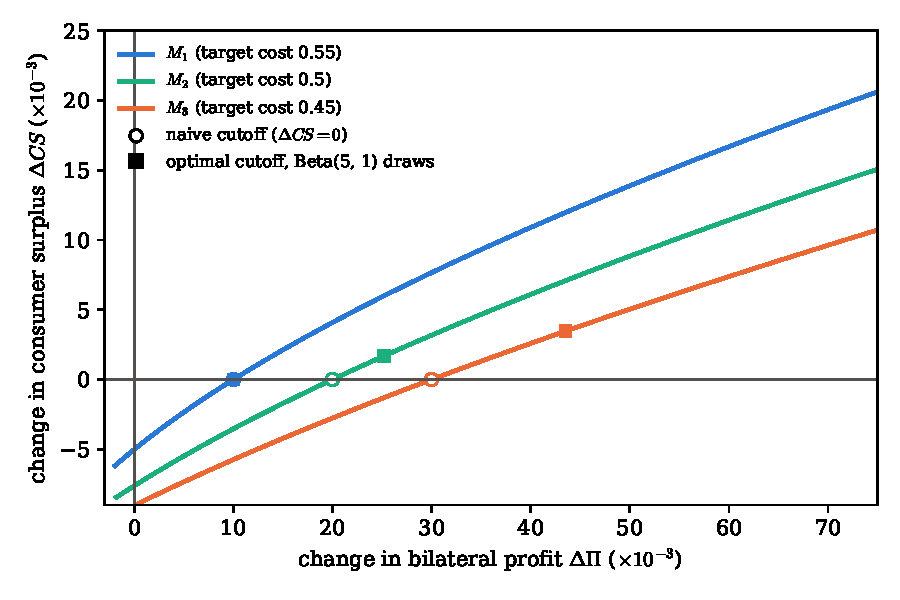
\includegraphics[width=0.78\textwidth]{figures/ch11/nw_curves.pdf}
\caption{Merger curves in $(\Delta\Pi, \Delta\mathit{CS})$ space for Example 2 of \citet{NockeWhinston2013}: inverse
demand $P = 1 - Q$, acquirer cost $c_0 = 0.5$ and targets with costs 0.55, 0.5 and 0.45. Each curve traces the outcomes
of one merger as the post-merger cost $\bar c_k$ varies from 0.2 to slightly above $c_k$. Open circles mark the naive
cutoffs, at which $\Delta\mathit{CS} = 0$. Squares mark the optimal cutoffs when post-merger costs follow the Beta(5, 1)
distribution described in the text. Our computation.}
\label{fig:11-nw}
\end{figure}

\subsection{The optimal approval policy}\label{sec:11-nw-optimal}

For a policy $\mathcal{A}$, let $\bar a_k = \max\mathcal{A}_k$ be the highest approved cost for target $k$. The merger
$(k, \bar a_k)$ is the \emph{marginal merger}, and $\underline{\Delta\mathit{CS}}_k = \Delta\mathit{CS}(k, \bar a_k)$ and
$\underline{\Delta\Pi}_k = \Delta\Pi(k, \bar a_k)$ are the lowest consumer surplus and profit changes among approved
mergers with target $k$.

The natural benchmark is the \emph{naive policy}, which approves every CS-nondecreasing merger, $\mathcal{A}_k = [c^L,
\hat c_k]$. It is not optimal. Suppose the authority tightens the standard for the largest merger $K$ only, approving it
only if $\Delta\mathit{CS} \ge \varepsilon$ for a small $\varepsilon > 0$. The two policies differ only when the naive
policy would lead to merger $K$ with $\Delta\mathit{CS} \in [0, \varepsilon)$. In that event, the naive policy delivers
at most $\varepsilon$. The tighter policy leads firms to propose the next most profitable acceptable merger, which
involves a smaller target. Its expected consumer surplus gain stays bounded away from zero as $\varepsilon \to 0$,
because some smaller merger is CS-increasing with positive probability. For small $\varepsilon$ the tighter policy
therefore does better. The main result characterizes the optimal policy.

\begin{proposition}[Optimal merger policy, \citealp{NockeWhinston2013}, Proposition 1]\label{prop:11-nw}
Any optimal approval policy has three properties. (i) It approves the smallest merger $M_1$ if and only if it is
CS-nondecreasing. (ii) It approves
with positive probability only mergers with targets in a set $\mathcal{K}^+ = \{1, \dots, \hat K\}$, where $\hat K$ may
equal $K$. (iii) It satisfies
\begin{equation}\label{eq:11-nw-prop1}
0 = \underline{\Delta\mathit{CS}}_1 < \underline{\Delta\mathit{CS}}_2 < \dots < \underline{\Delta\mathit{CS}}_{\hat K}.
\end{equation}
The minimum acceptable gain in consumer surplus is zero for the smallest merger, strictly positive for every larger
merger and increasing in the size of the merger. The largest mergers may never be approved.
\end{proposition}

\begin{proof}[Proof sketch]
The argument has six steps, each of which improves on a policy that violates a property.

Step 1. An optimal policy approves no CS-decreasing merger. Removing such mergers from $\mathcal{A}$ matters only when
one of them would have been proposed. Firms then propose another acceptable merger, which is CS-nondecreasing or the
status quo, so expected consumer surplus rises.

Step 2. Every CS-nondecreasing smallest merger is approved. Adding such mergers matters only when one of them becomes
the most profitable acceptable merger. Otherwise firms would propose the next most profitable acceptable merger, which
by Corollary~\ref{cor:11-nw} raises consumer surplus by less.

Step 3. The marginal merger satisfies an indifference condition. Let $E^{\mathcal{A}}_k(\bar a_k)$ be the expected
consumer surplus change from the merger firms would propose if $(k, \bar a_k)$ were rejected, conditional on $(k, \bar
a_k)$ being feasible and the most profitable acceptable merger. Then
\begin{equation}\label{eq:11-nw-indiff}
\underline{\Delta\mathit{CS}}_k = E^{\mathcal{A}}_k(\bar a_k).
\end{equation}
If the left side were smaller, rejecting mergers with costs just below $\bar a_k$ would raise expected consumer surplus.
If it were larger, approving mergers with costs just above $\bar a_k$ would raise it.

Step 4. Marginal profits increase with size: $\underline{\Delta\Pi}_j \le \underline{\Delta\Pi}_k$ for $j < k$ in
$\mathcal{K}^+$. If the order were reversed, some unapproved merger with target $j$ would give more consumer surplus
than the approved marginal merger with target $k$. Rejecting either leads to the same expected outcome, so approving the
first would help.

Step 5. Marginal consumer surplus increases strictly with size. Suppose $\underline{\Delta\mathit{CS}}_j \ge
\underline{\Delta\mathit{CS}}_k$ for $j < k$. By Step 3, $\underline{\Delta\mathit{CS}}_k$ equals the expected surplus of
the next most profitable acceptable merger. If that merger has profit between $\underline{\Delta\Pi}_j$ and
$\underline{\Delta\Pi}_k$, then by Step 4 it involves a smaller target and gives more than
$\underline{\Delta\mathit{CS}}_j$. If its profit is below $\underline{\Delta\Pi}_j$, then by Step 3 for target $j$ its
expected surplus is exactly $\underline{\Delta\mathit{CS}}_j$. The weighted average then exceeds
$\underline{\Delta\mathit{CS}}_j$, a contradiction.

Step 6. If target $j$ is never approved, no larger target is. The most efficient merger with $j$ gives more consumer
surplus than the most efficient merger with $j + 1$. Merging with the higher-cost target $j$ leaves a lower sum of
costs in the industry, hence more output. A nonmonotonicity argument
like that of Step 5 then applies. The appendix of the paper gives the formal proof.
\end{proof}

Proposition~\ref{prop:11-nw} gives the authority a reason to discriminate among mergers by a statistic it can observe
before any analysis. In the baseline model, a larger merger is one with a larger naive change in concentration,
$2s_0^0s_k^0$, and the optimal policy demands more from it. This rationale differs from the usual one for concentration
screens (\cref{sec:11-marketdef}). Higher concentration predicts larger harm in Cournot models, but here the screen
corrects for the bias in firms' choice of which merger to propose. The policy is a delegation rule. It accepts some
CS-increasing mergers with large targets less often than a merger-by-merger review would, in exchange for steering firms
toward the smaller mergers that consumers prefer.

\subsection{Cutoff policies, a numerical example and comparative statics}\label{sec:11-nw-cutoffs}

The indifference condition \eqref{eq:11-nw-indiff} links the policies for different targets, so it does not by itself
deliver the optimal policy. The problem simplifies if the optimal policy is a \emph{cutoff policy}, which approves merger
$k$ if and only if $\bar c_k \le \bar a_k$. Then the cutoffs follow by recursion. Set $\bar a_1 = \hat c_1$. For $k = 2,
\dots, K$, consider the best acceptable merger among targets $1, \dots, k - 1$, conditional on its profit being at most
$\Delta\Pi(k, \bar a_k)$. Set $\bar a_k$ at the largest cost at which $\Delta\mathit{CS}(k, \bar a_k)$ equals the
expected consumer surplus from that merger. If no such cost exists, merger $k$ and all larger mergers are never approved.

The optimal policy need not have this form. In Example 1 of the paper, the smaller merger is always feasible and gives
$(\Delta\Pi, \Delta\mathit{CS}) = (5, 5)$ with probability 0.9 and $(1, 1)$ with probability 0.1, so its expected
consumer surplus gain is $0.9 \times 5 + 0.1 \times 1 = 4.6$.\footnote{The text of the paper attaches probability 0.9
to the outcome $(1, 1)$. Its Figure 8 and its value of 4.6 require probability 0.9 on $(5, 5)$.} The larger merger's curve passes through $\Delta\mathit{CS} = 4.6$ before it reaches
$\Delta\Pi = 5$. For costs between these two points the larger merger would always be proposed, yet it would give less
than 4.6. The authority rejects it there and approves it at both higher and lower costs, so the approval set is not an
interval. Proposition~2 of the paper gives a sufficient condition, checkable in applications, under which the recursive
cutoff policy is optimal.

\begin{example}[Nocke and Whinston's Example 2]\label{ex:11-nw}
Let $P(Q) = 1 - Q$ and four firms have costs $c_0 = c_2 = 0.5$, $c_1 = 0.55$ and $c_3 = 0.45$. With four Cournot firms,
$Q^0 = \frac{4 - 2}{5} = 0.4$ and $P^0 = 0.6$. Outputs are $P^0 - c_i$, so pre-merger shares are $\frac{1}{4}$,
$\frac{1}{8}$, $\frac{1}{4}$ and $\frac{3}{8}$. The naive cutoffs are $\hat c_k = c_k - (P^0 - c_0) = c_k - 0.1$, that is,
0.45, 0.40 and 0.35. Each merger is feasible with probability $\phi_k = 0.75$. Conditional on feasibility, $\bar c_k =
0.2 + (\hat c_k - 0.2)X$, where $X$ follows a Beta distribution with density proportional to $x^{\alpha_B - 1}$ on $[0,
1]$. A larger shape parameter $\alpha_B$ makes small efficiency gains more likely. The lower bound 0.2 keeps every firm
active.
\end{example}

\Cref{tab:11-nwex} reports the paper's results with our replication. We compute the recursive cutoffs by simulating 2
million draws of the feasible set and solving the indifference condition with a root finder. For $\alpha_B = 5$, the
optimal cutoffs are $\bar a_2 = 0.383$ and $\bar a_3 = 0.316$, well below the naive 0.40 and 0.35. The optimal policy
requires the medium merger to raise consumer surplus by 0.00170 and the large merger by 0.00346. It achieves 90.3 percent
of the first-best gain, which a fully informed authority choosing the best feasible merger would obtain, while the naive
policy achieves 79.8 percent. As $\alpha_B$ falls, large efficiencies become more likely, the first-best gain rises and
the advantage of the optimal policy over the naive one shrinks.

\begin{table}[htbp]
\centering
\caption{Optimal and naive merger policies in the linear example}
\label{tab:11-nwex}
\begin{threeparttable}
\small
\setlength{\tabcolsep}{4.5pt}
\begin{tabular}{@{}llccccccc@{}}
\toprule
$\alpha_B$ & Source & $\bar a_2$ & $\bar a_3$ & $\underline{\Delta\mathit{CS}}_2$ & $\underline{\Delta\mathit{CS}}_3$ &
\makecell{First-best gain\\ (\% of $\mathit{CS}^0$)} & \makecell{Naive\\ (\% of first best)} &
\makecell{Optimal\\ (\% of first best)} \\
\midrule
5 & Paper & 0.383 & 0.316 & 0.00170 & 0.00346 & 6.44 & 79.83 & 90.30 \\
 & Replication & 0.383 & 0.316 & 0.00170 & 0.00346 & 6.44 & 79.83 & 90.27 \\
3 & Paper & & & 0.00170 & 0.00457 & 9.55 & 87.34 & 92.13 \\
 & Replication & 0.383 & 0.305 & 0.00170 & 0.00457 & 9.55 & 87.35 & 92.15 \\
1 & Paper & & & 0.00099 & 0.00571 & 18.15 & 93.67 & 94.10 \\
 & Replication & 0.390 & 0.294 & 0.00098 & 0.00573 & 18.14 & 93.67 & 94.12 \\
\bottomrule
\end{tabular}
\begin{tablenotes}[flushleft]
\footnotesize
\item Notes: Paper rows from \citet[Example 2 and Table 1]{NockeWhinston2013}, which report cutoffs only for $\alpha_B = 5$
and write $\alpha$ for the shape parameter. The smallest merger's cutoff is the naive one, $\bar a_1 = 0.45$, with
$\underline{\Delta\mathit{CS}}_1 = 0$. Replication rows are our Monte Carlo computation with 2 million simulated feasible
sets. Differences in the last digit reflect simulation error.
\end{tablenotes}
\end{threeparttable}
\end{table}

When the optimal policy has a cutoff form, two comparative statics follow (Propositions 3 and 4 of the paper). First, if
merger $k$ becomes less likely to be feasible, the standards for mergers up to $k$ do not change, and the standards for
larger approved mergers fall. A less likely alternative makes rejection less valuable, so the authority can be more
lenient. As all feasibility probabilities go to zero, the optimal policy approaches the naive one. Second, if the
acquirer becomes more efficient, all cost cutoffs fall. The authority then demands lower post-merger costs from every
merger.

\subsection{Extensions}\label{sec:11-nw-ext}

Section~5 of the paper shows that the main result survives five changes to the model.

\emph{Other bargaining processes.} The offer game gives firm 0 the whole bilateral gain. The same proposals arise if
firm 0 obtains a fixed share of the gain from every target, as in alternating-offer bargaining with a common discount
factor. With efficient bargaining among all firms, the proposed merger maximizes aggregate profit instead. Part (iv) of
\cref{lem:11-nw1} still holds, and a version of \cref{lem:11-nw3} holds for aggregate profit. \Cref{lem:11-nw2} needs
an extra assumption, that a lower
post-merger cost raises aggregate profit for CS-nondecreasing mergers. The same conclusions hold if only a subset of
firms that includes all merger candidates bargains efficiently.

\emph{General sets of mergers.} Suppose mergers may involve any set of firms, with $m_k \ge 2$ partners, and bargaining is
efficient. Summing first-order conditions shows that aggregate profit is proportional to the post-merger Herfindahl
index,
\begin{equation}\label{eq:11-nw-aggprofit}
\sum_i \pi_i(M_k) = \sum_i -P'(Q)\,q_i^2 = \big|Q^2P'(Q)\big|\, \HHI(M_k),
\end{equation}
where we used $\pi_i = -P'q_i^2$ from \eqref{eq:11-nw-profit}. For a CS-neutral merger, outputs of nonmerging firms are
unchanged, so the actual post-merger index equals the naive one, $\HHI(M_k) = \HHI^{naive}(M_k)$. Among CS-neutral mergers,
the one with the higher naive post-merger Herfindahl index therefore raises aggregate profit more. Under conditions that
make merger curves upward sloping and non-crossing, the authority should discriminate by the naive post-merger index.
This is the statistic that concentration screens in merger guidelines use (\cref{tab:11-guidelines}).

\emph{Differentiated products.} With CES or logit demand and price competition, profits can be written as functions of
a firm's own strategic variable and an aggregator $\Psi = \sum_j\psi_j$. Its terms are unrelated to the curvature
$\psi$ of \cref{sec:11-passthrough}, and consumer surplus increases with $\Psi$.
For logit demand $\psi_j = \exp\big(\alpha(\bar v - p_j)\big)$ and consumer surplus is $\frac{1}{\alpha}\ln\Psi$ plus a
constant, as in \cref{ch:logit}. For CES demand with elasticity of substitution $\varsigma > 1$, $\psi_j = p_j^{1 - \varsigma}$.
These aggregative games share the properties of the Cournot model that \cref{lem:11-nw1,lem:11-nw2,lem:11-nw3} use,
so \cref{prop:11-nw} carries over. \citet{NockeSchutz2018} develop the aggregative-games approach for multiproduct
firms, which \cref{sec:11-fs} used to extend the synergy condition beyond Cournot.

\emph{Other welfare standards.} If the authority maximizes $W = \mathit{CS} + \omega\,\Pi$ with $\omega \in [0, 1]$,
where $\omega = 1$ is the total surplus standard, the analogue of \cref{prop:11-nw} holds under efficient bargaining. The
minimum acceptable welfare gain is zero for the smallest merger and rises with size. For the offer game, the result holds
when $\omega$ is small.

\emph{Fixed-cost synergies.} If mergers also save fixed costs, merger curves become bands. The main result holds when the
idiosyncratic fixed-cost savings are small enough that bands of different mergers do not overlap. Common fixed-cost
savings shift all bands equally and leave the optimal policy unchanged.

\subsection{Lessons and limits}\label{sec:11-nw-lessons}

Two lessons stand out. First, a merger-by-merger consumer surplus test is not the best policy when firms choose among
mutually exclusive mergers. The authority should ask what the alternative merger would have been, not only what the
proposed merger does. Second, naive concentration statistics carry information about firms' proposal incentives, which
gives screens based on $2s_0s_k$ and the naive post-merger index a rationale beyond their role as predictors of price
effects.

Later work gives the naive change a second rationale, which \cref{sec:11-hhi} reports. With price competition under
logit, nested logit or CES demand, the consumer surplus lost in a merger without synergies is approximately
proportional to the naive $\Delta\HHI$ \citep{NockeSchutz2019}. The efficiencies needed to leave consumers unharmed
rise with the naive change and, holding it fixed, do not depend on the level of the index \citep{NockeWhinston2020}.
The Cournot version of this result is \eqref{eq:11-required-dhhi}. Both rationales point to naively computed
concentration statistics, and the second singles out the change. \citet{NockeWhinston2020} also conclude that the
presumptions of the 2010 Guidelines are likely too lax \citep[p.~227, n.~124]{AskerNocke2021}.

The model's limits are also clear. The authority commits to a policy and observes everything about the proposed merger,
including post-merger costs, which in practice must be predicted. Only one merger can be proposed, and the setting is
static. In a dynamic world, mergers rejected today may be replaced by others tomorrow, and approved mergers change the
pool of future mergers. \citet{NockeWhinston2010} show that when possible mergers are disjoint, a myopic consumer surplus
standard is optimal, so the force identified here comes from overlap among possible mergers. The next subsection
explains why.

\subsection{Merger review over time, investment and innovation}\label{sec:11-dynamics}

Mergers are not one-time events. When merger opportunities arise over time, approving a merger today changes the
profitability and the welfare effects of the mergers that rivals may propose later \citep[p.~232]{AskerNocke2021}. A
policy that looks only at current market conditions may then be wrong. This subsection shows when it is not, and what
changes once firms invest and innovate.

\casehead{A complementarity between disjoint mergers}
Two mergers are \emph{disjoint} if no firm takes part in both. In the Cournot model of \cref{sec:11-nw-model}, the
consumer surplus effects of disjoint mergers have a simple structure.

\begin{proposition}[Sign-preserving complementarity, \citealp{NockeWhinston2010}]\label{prop:11-signpreserve}
Let inverse demand satisfy \eqref{eq:11-nw-ass}, let marginal costs be constant, and let all firms be active in every
market structure considered. Let $\mathcal{M}_A$ and $\mathcal{M}_B$ be disjoint mergers with post-merger costs
$c_A$ and $c_B$.
\begin{enumerate}[label=(\roman*)]
\item If each merger is CS-nondecreasing at the current market structure, each remains CS-nondecreasing once the other
has taken place.
\item If each merger is CS-decreasing at the current market structure, each remains CS-decreasing once the other has
taken place.
\end{enumerate}
\end{proposition}

\begin{proof}
With constant marginal costs, \cref{prop:11-synergy-gen} says that a merger $\mathcal{M}$ with post-merger cost
$c_{\mathcal{M}}$ is CS-nondecreasing at a market structure with price $P$ if and only if
\begin{equation*}
P - c_{\mathcal{M}} \ge \sum_{i \in \mathcal{M}}(P - c_i) = |\mathcal{M}|\,P - \sum_{i \in \mathcal{M}}c_i .
\end{equation*}
Rearranging,
\begin{equation}\label{eq:11-cs-cutoff-P}
c_{\mathcal{M}} \le \sum_{i \in \mathcal{M}}c_i - \big(|\mathcal{M}| - 1\big)P .
\end{equation}
The right side falls in $P$, because $|\mathcal{M}| \ge 2$. Let $P^0$ be the current price and $P^B$ the price after
$\mathcal{M}_B$. The good is homogeneous, so $P^B \le P^0$ if $\mathcal{M}_B$ is CS-nondecreasing and $P^B > P^0$ if it is
CS-decreasing. The partners of $\mathcal{M}_A$ are not in $\mathcal{M}_B$, so their costs and $c_A$ do not change.
Only the price in \eqref{eq:11-cs-cutoff-P} moves. In case (i), \eqref{eq:11-cs-cutoff-P} holds for $\mathcal{M}_A$ at
$P^0$, and its right side weakly rises when the price falls to $P^B$. So it still holds. In case (ii),
\eqref{eq:11-cs-cutoff-P} fails for $\mathcal{M}_A$ at $P^0$, and its right side falls when the price rises to $P^B$. So
it still fails. Exchanging the roles of the two mergers completes the proof.
\end{proof}

The intuition is that a merger is more likely to help consumers the more intense competition is, because intense
competition weakens its market-power effect. A CS-increasing merger intensifies competition. It can even turn a second,
CS-decreasing merger into a CS-increasing one, and the first merger then stays CS-increasing once the second has taken
place \citep[p.~233]{AskerNocke2021}.

\casehead{Myopic review can be optimal}
\Cref{prop:11-signpreserve} underlies the dynamic result of \citet{NockeWhinston2010}. Suppose merger opportunities
arrive over time, a merger that is not proposed or is blocked today can be proposed again later, and possible mergers
are disjoint. An authority that maximizes discounted consumer surplus can then adopt a completely myopic policy. In each
period it approves the subset of proposed mergers that maximizes current consumer surplus and ignores future mergers.
It never regrets approving a merger that is CS-nondecreasing when approved, by part (i). It never regrets blocking a
CS-decreasing merger, because the opportunity remains and the merger can be approved once its effect turns positive.
Firms' incentives to propose are aligned with the authority's goal, because a CS-nondecreasing merger is profitable
(\cref{cor:11-neutral-profit}) and stays profitable when it induces other mergers. The myopic policy is optimal in a
strong sense. The authority could not do better even with perfect foresight of future merger opportunities and the
power to undo past approvals \citep[p.~233]{AskerNocke2021}. The result extends to price competition with logit or CES
demand \citep{NockeSchutz2019}.

Both assumptions matter. When firms choose among alternative partners, as in \cref{sec:11-nw-model}, possible mergers
overlap and are not disjoint. That is why approving every CS-nondecreasing merger is optimal in
\citet{NockeWhinston2010} but not in \citet{NockeWhinston2013} \citep[p.~234, n.~141]{AskerNocke2021}.

\casehead{Investment, entry and buyouts}
\citet{MermelsteinEtAl2020} compute optimal merger policy in a dynamic model with scale economies. Firms lower their
unit costs by accumulating capital, and mergers lower them by combining capital stocks. Firms choose investment and
whether to propose a merger, and the authority decides whether to block it. After an approved merger, a potential
entrant without capital appears and decides how much to invest. Three findings stand out \citep[pp.~235--236]{AskerNocke2021}.
First, the optimal dynamic policy differs markedly from the static policy that evaluates each merger at the current
state. Second, commitment matters. If society values discounted aggregate surplus but the authority cannot commit to
its future policy, giving it a tougher consumer surplus standard can be better. Third, in their baseline a permissive
policy raises firms' incentives to invest in almost every state, yet it lowers investment on average. Once mergers are
allowed, the industry spends more time in concentrated states, where incentives to invest are weak. A permissive policy
also induces entry for buyout, in which entrants overinvest in capital only to be bought by an incumbent
\citep{Rasmusen1988}.

A static model gives a sharper result for process innovation. \citet{MottaTarantino2019} let each firm choose its price
and an investment that lowers its marginal cost, with demand that has the independence of irrelevant alternatives
property. Suppose the merger's synergies affect production costs and not the cost of investment. If the merging
partners want to raise their prices at the pre-merger investments, they also want to invest less, because the return to
a lower marginal cost grows with output. A merger that leaves consumers unharmed therefore requires the same production
cost synergies as when investment is ignored \citep[pp.~234--235]{AskerNocke2021}.

\casehead{Innovation}
Acquisitions of innovative rivals raise a different question. \citet{Cabral2018} studies a dominant firm and a fringe
firm that invest in innovation over time. An acquisition transfers the leader's technology to the laggard. In
equilibrium the dominant firm acquires the fringe firm's innovations, and allowing such acquisitions raises the rate of
incremental innovation, an \emph{innovation for buyout} effect. When firms can also invest in radical innovation, which
would make the fringe firm dominant, acquisitions lower the radical innovation rate \citep[p.~236]{AskerNocke2021}.
\citet{IgamiUetake2019} provide rare empirical evidence. They estimate a dynamic model of the hard disk drive
industry with endogenous innovation, entry and exit. In their model, the rule of thumb that blocks mergers when three
or fewer firms exist comes reasonably close to maximizing the discounted value of social welfare
\citep[p.~264]{AskerNocke2021}. \Cref{sec:11-open} returns to acquisitions that end innovation projects.

\section{Assessment and open issues}\label{sec:11-discussion}

\subsection{What the approaches deliver}\label{sec:11-approaches}

This chapter has studied three families of tools. Retrospective studies compare prices before and after consummated
mergers with a control group, using difference-in-differences or stock-market event studies (\cref{sec:11-retro}).
Simple theory, through upward pricing pressure and its relatives, turns diversion ratios and margins into a screen
(\cref{sec:11-upp}). Prospective econometric models estimate demand, recover costs from first-order conditions and
solve for the post-merger equilibrium (\cref{sec:11-simulation}). \Cref{tab:11-approaches} summarizes what each requires
and where the evidence of this chapter shows its weaknesses.

\begin{table}[htbp]
\centering
\caption{Approaches to evaluating horizontal mergers}
\label{tab:11-approaches}
\begin{threeparttable}
\footnotesize
\begin{tabularx}{\textwidth}{@{}>{\raggedright\arraybackslash}p{2.3cm}>{\raggedright\arraybackslash}X%
>{\raggedright\arraybackslash}X>{\raggedright\arraybackslash}X@{}}
\toprule
Approach & What it needs & What it delivers & Weaknesses seen in this chapter \\
\midrule
Retrospective difference-in-differences & Prices of merging firms and a control group before and after a
consummated merger & Transparent estimate of the realized price effect & Controls react strategically (Houde,
Analgesics). Samples and price measures matter (Hastings versus Taylor et al.). Only cleared mergers are observed \\
\addlinespace
Stock-market event studies & Abnormal returns of merging firms and rivals & Market expectations of profits &
Profits, not consumer effects. Confounding news \\
\addlinespace
Upward pricing pressure and GUPPI & Diversion ratios, margins, an efficiency credit & Sign of the price pressure
without market definition & Magnitudes require pass-through and hence demand curvature \\
\addlinespace
Merger simulation & Estimated demand, a conduct assumption and equilibrium computation & Price, quantity and welfare
predictions for any counterfactual & Functional form drives pass-through (Analgesics). Logit shocks dampen rival
responses (Houde). Conduct may change (MillerCoors). Products and capacity held fixed \\
\addlinespace
Models of repositioning, investment and merger choice & Product or capacity choices before and after mergers & Effects
beyond short-run prices & Mostly descriptive (Sweeting). Costs inferred as residuals (Pesendorfer). Policy models
assume commitment and observability (Nocke and Whinston) \\
\bottomrule
\end{tabularx}
\begin{tablenotes}[flushleft]
\footnotesize
\item Notes: Our summary. Analgesics refers to \citet{BjornerstedtVerboven2016}, MillerCoors to
\citet{MillerWeinberg2017}, and Taylor et al.\ to \citet{TaylorKreisleZimmerman2010}.
\end{tablenotes}
\end{threeparttable}
\end{table}

The approaches are complements. Retrospective estimates validate or reject the assumptions of structural models, as in
\citet{Houde2012} and \citet{BjornerstedtVerboven2016}. Structural models explain what retrospective designs can and
cannot identify, such as the bias from contaminated controls. Simple screens are cheap and robust in sign but say little
about magnitudes. The validation record is mixed. Houde's simulation matches the retrospective magnitude, while
analgesics simulations with unit demand under-predict the price increase, and simulations of airline mergers show large
prediction errors \citep{Peters2006}.
The MillerCoors evidence suggests that post-merger conduct may change in ways a unilateral-effects simulation misses.

\subsection{Limitations of current practice}\label{sec:11-limits}

Three limitations recur. The first is the focus on price. Mergers also change quality, branding and variety. Merging
radio stations repositioned their playlists without changing their commercial loads (\cref{sec:11-sweeting}). After
Maytag-Whirlpool the merged firm cut the number of models it offered (\cref{sec:11-maytag}). Price-only evaluations miss
these margins, and their welfare effects are hard to sign (\cref{ch:newgoods}).

The second is the static framing. Standard analysis holds fixed entry, capacity and the pool of future mergers.
Pesendorfer's model shows that investment responses can make mergers without synergies profitable and raise their price
effects. Nocke and Whinston show that the optimal standard depends on the alternatives firms could have chosen. Dynamic
models of mergers with entry and investment \citep{BerryPakes1993,Gowrisankaran1999,MermelsteinEtAl2020} and dynamic
merger review \citep{NockeWhinston2010} address these issues, at the cost of heavy computation and many assumptions
(\cref{sec:11-dynamics}). Free entry, the static benchmark for these concerns, is slow in practice
(\cref{sec:11-freeentry}).

The third is the choice of industries. Most of the evidence comes from markets with good scanner or survey data and
fairly simple products: cereal, beer, analgesics, gasoline and appliances. Many contested mergers involve hospitals,
platforms, technology, networks or inputs sold through negotiation. In these markets prices are bargained, products are
complex, or one side of the market pays nothing. Bargaining changes the analysis. \citet{GowrisankaranNevoTown2015}
show that insurers' bargaining power can substantially counteract the market power of merging hospitals
(\cref{sec:11-dafny}). \citet{LoertscherMarx2019} study bidding markets in which a powerful buyer runs a procurement
auction. As in \citet{FarrellShapiro1990}, a merger of suppliers without cost synergies harms the buyer, although buyer
power mitigates the harm. Strong synergies can remove the harm, but they can also make an otherwise profitable merger
unprofitable \citep[p.~238]{AskerNocke2021}.

\subsection{Remedies}\label{sec:11-remedies}

Authorities approve mergers subject to remedies far more often than they block them. From 1990 to 2014 the European
Commission approved about 15 times as many mergers with remedies as it prohibited. In the United States, 60 percent of
the mergers that the agencies challenged between 2003 and 2012 were later approved with remedial commitments
\citep[p.~253]{AskerNocke2021}. A \emph{behavioral remedy} constrains the merged firm's conduct, for example through a
licensing agreement. A \emph{structural remedy}, or \emph{divestiture}, transfers physical assets or intellectual property
to another firm. Given how common remedies are, surprisingly little is known about them. Whether a divestiture
eliminates the harm of a merger depends on how the transferred assets change the costs of the buyer and of the merged
firm. It also depends on how the divestiture interacts with any synergies.

\casehead{When divestitures help}
\citet{Verge2010} studies a Cournot model in which every firm has the same cost function $C(q, k)$, homogeneous of
degree one in output and capital. A merger without synergies pools the partners' capital and is CS-decreasing. A
divestiture moves some of the merged firm's capital to outsiders. Vergé shows that divestitures mitigate the harm to
consumers if and only if the reallocation makes the industry more symmetric. He also shows when no divestiture can
restore pre-merger consumer surplus, which depends on the number of outsiders and on the pre-merger asymmetries in
capital \citep[pp.~253--254]{AskerNocke2021}.
The physical-capital technology of \cref{ex:11-fs-tech}, $C(q, k) =
\frac{q^2}{2k}$, is homogeneous of degree one and shows the mechanism. Industry output is $Q = \frac{a\tilde K}{1 +
\tilde K}$, which rises with
\begin{equation*}
\tilde K = \sum_i g(k_i), \qquad g(k) = \frac{k}{1 + k} .
\end{equation*}
The function $g$ is strictly concave with $g(0) = 0$, so consumer surplus is a concave function of the distribution of
capital. Without a divestiture, the merger of firms 1 and 2 changes $\tilde K$ by $g(k_1 + k_2) - g(k_1) - g(k_2) < 0$,
since a strictly concave function with $g(0) = 0$ is strictly subadditive. Now let the merged firm, with capital $k_M =
k_1 + k_2$, transfer an amount $d$ to an outsider $o$. The change in $\tilde K$ relative to the merger without divestiture is
\begin{equation*}
\Gamma(d) = g(k_M - d) + g(k_o + d) - g(k_M) - g(k_o),
\qquad
\Gamma'(0) = g'(k_o) - g'(k_M) .
\end{equation*}
Because $g'$ is decreasing, $\Gamma'(0) > 0$ if and only if $k_o < k_M$. A small divestiture therefore raises
consumer surplus if and only if it goes to a firm smaller than the merged firm. In other words, it must make the two
firms more alike. Since $\Gamma$ is concave, the best divestiture to a single smaller outsider equalizes the two capital stocks.
With three firms of capital 1, for instance, $\tilde K = 1.5$ before the merger. The merged firm has capital 2, and
the best divestiture of $\frac{1}{2}$ leaves two firms with capital 1.5 each and $\tilde K = 2 \times 0.6 = 1.2$. This is
above the 1.17 of the merger without remedy, $g(2) + g(1) = \frac{2}{3} + \frac{1}{2}$, and below the pre-merger 1.5. The
divestiture mitigates the harm without removing it. These results concern unilateral effects. With coordinated effects they may reverse,
since asymmetries hinder collusion (\cref{prop:11-cjr}).

\citet{NockeRhodes2019} study remedies for mergers that span many markets. In each market the partners hold assets
that can be divested to outsiders, including firms not yet active. The set of divestitures is the outcome of efficient
bargaining between an authority that cares about consumer surplus and the profit-maximizing partners. It is subject to
a consumer surplus constraint in each market and to the partners' participation constraint. More competitive markets
need fewer divestitures. The key concept is the \emph{remedies exchange rate}, the profit the merged firm must give up
for an extra dollar of consumer surplus. Under conditions on the curvature of demand, the rate improves in a market as
more assets are divested there. The efficient bargain is then bang-bang: maximum divestitures in some markets and only
the minimum needed to meet the constraint in the others. Perhaps surprisingly, the efficient bargain places the
maximum divestitures in the markets where the partners face more efficient rivals. The reason is that the average
remedies exchange rate tends to be worse in those markets \citep[p.~254]{AskerNocke2021}.

\casehead{Evidence}
\citet{FribergRomahn2015} study the 2001 merger of Carlsberg and Pripps in the Swedish beer market. The authority
approved it on condition that the partners divest 18 beer varieties to a small rival, Galatea. A
difference-in-differences comparison with the non-merging brewers as controls shows that the merger with remedies
lowered the prices both of the partners' retained varieties and of the divested ones. The first result suggests
synergies large enough to outweigh market power. The second fits a buyer with less market power than the partners had
before the merger. A random-coefficients logit simulation on pre-merger data predicts that, without cost changes, the
divestitures would have reduced the price increases of the retained products without eliminating them. Post-merger
prices imply marginal cost savings of 5 percent for Carlsberg and 10 percent for Pripps \citep[p.~255]{AskerNocke2021}.
Two caveats apply. The non-merging brewers may be invalid controls, and the merger was anticipated long before it was
consummated, so there is no sharp break between the periods (n.~197). \citet{Lagos2018} studies station divestitures
after a 2013 merger in Chilean retail gasoline. Where the merger raised concentration, retail margins rose by between
0 and 4 percent depending on the specification. Stations within 1 kilometer of a divested station saw margins fall by
about 2 percent, but only in municipalities with few affected stations \citep[p.~263]{AskerNocke2021}. In their
conclusion, \citet[p.~261]{AskerNocke2021} single out the effects of divestitures and their optimal design as an area
where little is known.

\subsection{Recent controversial mergers}\label{sec:11-recent}

\Cref{tab:11-recent} lists proposed mergers that drew public controversy in the decade and a half before this edition.
They span health care, telecommunications and media, retail, airlines, technology, finance and rail. Several raise
issues that the tools of this chapter address only partly.

\begin{table}[htbp]
\centering
\caption{Selected controversial proposed mergers in the United States}
\label{tab:11-recent}
\begin{threeparttable}
\small
\begin{tabularx}{\textwidth}{@{}>{\raggedright\arraybackslash}p{2.9cm}>{\raggedright\arraybackslash}p{5.4cm}%
>{\raggedright\arraybackslash}X@{}}
\toprule
Sector & Proposed merger & Outcome \\
\midrule
Health care & Aetna and Humana & Blocked, 2017 \\
 & Anthem and Cigna & Blocked, 2017 \\
 & UnitedHealth and Amedisys & Allowed with divestitures, 2025 \\
 & Edwards Lifesciences and JenaValve & Blocked by preliminary injunction, 2026 \\
\addlinespace
Telecom and media & AT\&T and T-Mobile & Abandoned, 2011 \\
 & Comcast and Time Warner Cable & Abandoned, 2015 \\
 & T-Mobile and Sprint & Allowed, 2020 \\
 & Paramount and Warner Bros.\ Discovery & Cleared by the DOJ, then challenged by 12 states and settled by consent
decree, 2026 \\
\addlinespace
Retail and airlines & Kroger and Albertsons & Blocked, 2024 \\
 & Tapestry and Capri & Blocked, 2024 \\
 & JetBlue and Spirit & Blocked, 2024 \\
\addlinespace
Technology and finance & Microsoft and Activision Blizzard & FTC challenge failed, 2023 \\
 & Capital One and Discover & Allowed, 2025 \\
 & Hewlett Packard Enterprise and Juniper & DOJ settlement, entered by the court in 2026 after a contested Tunney Act
review \\
\addlinespace
Rail & Union Pacific and Norfolk Southern & Under Surface Transportation Board review, final briefs due May 2027 \\
\bottomrule
\end{tabularx}
\begin{tablenotes}[flushleft]
\footnotesize
\item Notes: Status as of autumn 2026. The Tunney Act (Antitrust Procedures and Penalties Act) requires a court to find
that a consent decree negotiated by the Department of Justice is in the public interest. The Surface Transportation Board
has exclusive jurisdiction over railroad mergers. Outcomes from 2025 on follow the agencies' orders and settlements and
the courts' opinions and orders.
\end{tablenotes}
\end{threeparttable}
\end{table}

\subsection{Open issues}\label{sec:11-open}

The cases in \cref{tab:11-recent} point to several issues that a complete merger analysis must handle.

\emph{Two-sided platforms and media.} Media and payment networks serve two groups whose participation affects each
other. A merger can raise the price to one side and lower it to the other, and the relevant welfare measure combines
both. Radio is an example, where \citet{Sweeting2010} studied listeners while the Department of Justice examined
advertising prices. Structural analyzes of media mergers with two-sided demand include \citet{ChandraCollardWexler2009}
and \citet{Jeziorski2014}. Platform economics lies outside the scope of this edition.

\emph{Labor-market power.} Mergers of employers can lower wages where workers have few alternative employers, as in
hospitals or grocery chains. \citet{PragerSchmitt2021} find slower wage growth for skilled hospital workers after
mergers that substantially raised employer concentration. The tools of this chapter carry over with labor supply in place
of product demand, and the 2023 Merger Guidelines discuss labor markets explicitly \citep{USDOJFTC2023}.

\emph{Innovation and nascent competition.} In technology and pharmaceuticals, a target may be a small firm whose future
products could challenge the acquirer. \citet{CunninghamEdererMa2021} show that incumbent drug firms acquire projects that
overlap with their own and then discontinue them more often than other projects. Current prices say little about such
losses, and predicting the counterfactual development path is hard.

\emph{Failing firms, capacity and networks.} Airline mergers combine networks and capacity, and their effects depend on
route-level overlap, hub dominance and entry (\cref{ch:airlines}). Arguments that a target would exit without the merger,
raised for example in airline cases, require a counterfactual in which the target's assets leave the market.

\emph{Vertical and complementary effects.} Several cases combine horizontal overlaps with vertical relations, such as
content and distribution in media or devices and network equipment. Foreclosure and the elimination of double
marginalization then enter alongside unilateral effects. \citet{Houde2012} illustrates how vertical control of retail
prices can turn a supply agreement into a horizontal merger in effect.

\emph{Remedies.} Divestitures and behavioral commitments aim to preserve competition while allowing efficiencies.
\Cref{sec:11-remedies} shows that their theory is young and their evidence thin. The Tunney Act review of Department
of Justice settlements makes the design of remedies a legal issue as well.

\emph{Rising markups and common ownership.} Two aggregate literatures form a backdrop to merger policy
\citep[pp.~257--261]{AskerNocke2021}. \citet{DeLoeckerEeckhoutUnger2020} estimate the markups of US publicly listed
firms from 1955 to 2016, following the production approach of \citet{DeLoeckerWarzynski2012}. The revenue-weighted
average rises, but most firms see no increase and the median is flat. The rise comes from the upper tail. Between
1980 and 2016 the 90th-percentile markup rose from 1.5 to 2.5. The second literature measures \emph{common ownership},
the holding of equity in competing firms by the same institutional investors. \citet{BackusConlonSinkinson2021a}
compute the weight that each S\&P 500 firm would place on every other firm's profit if managers served their common
owners. The mean weight across pairs rose from about 0.2 in 1980 to almost 0.7 in 2017. These weights are the
off-diagonal $\kappa_{fg}$ of the objective \eqref{eq:11-mc-objective} and the matrix $\Omega(\kappa)$ of
\cref{prop:11-mc-foc}, read literally as ownership shares in the sense of \citet{OBrienSalop2000}. A rise in common
ownership thus acts like a partial merger among the firms' owners, without a filing or a review. Whether it changes
conduct in product markets is still debated.

\emph{Regulated industries and political economy.} Rail mergers are reviewed by the Surface Transportation Board under a
public-interest standard, outside the Clayton Act framework of \cref{sec:11-review}. State attorneys general can sue to block
mergers that federal agencies cleared. These institutions change which mergers are proposed and how they are judged. In
the spirit of \cref{sec:11-policy}, they also change firms' incentives over which merger to propose.
